\documentclass[a4paper,12pt]{report}
\usepackage[utf8]{inputenc}
\usepackage{amsmath, amssymb}
\usepackage{geometry}
\geometry{margin=1in}
\usepackage{graphicx}
\usepackage{hyperref}
\usepackage{titlesec}
\usepackage{fancyhdr}
\usepackage{xeCJK}
\usepackage{fontspec}
\usepackage{enumitem} % 支援題庫的 enumerate
\usepackage{tikz} % 繪圖
\usepackage{pgfplots} % 繪圖
\usepackage{physics} % 物理符號
\usepackage{listings} % 程式碼
\usepackage{circuitikz}


% 修正 headheight 警告
\setlength{\headheight}{15pt}
\addtolength{\topmargin}{-3pt}

% 設定標楷體
\setCJKmainfont[
    AutoFakeBold = {2.0}
]{AR PL UKai TW}

% 兼容不同系統
\IfFileExists{C:/Windows/Fonts/kaiu.ttf}{
    \setCJKmainfont{DFKai-SB}
}{
    \IfFileExists{/System/Library/Fonts/Supplemental/BiauKai.ttf}{
        \setCJKmainfont{BiauKai}
    }{
        \setCJKmainfont{AR PL UKai TW}
    }
}

% 標題格式
\titleformat{\chapter}{\Huge\bfseries}{\thechapter}{1em}{}
\titleformat{\section}{\Large\bfseries}{\thesection}{1em}{}

% 頁眉
\pagestyle{fancy}
\fancyhf{}
\fancyhead[L]{數A滿級分講義}
\fancyhead[R]{\thepage}

\title{數A滿級分講義}
\author{Your Name}
\date{\today}

\begin{document}

\maketitle
\tableofcontents

\chapter*{前言}
\addcontentsline{toc}{chapter}{前言}

\section*{講義目標}
本講義旨在幫助考生全面掌握台灣大學入學學力測驗(學測)數學A的考試範圍,並以追求滿級分為目標。學測數學A的特點在於「觀念熟悉但題目新穎」,因此我們不僅深入講解每個單元的基礎知識,還融入大學層次的解題技巧,讓你在考場上能快速應對各種變化。無論你是自然組的考生還是自學者,這份講義都將成為你通往高分的利器。

\section*{講義特色}
\begin{itemize}
    \item \textbf{觀念深度}:從108課綱的高中數學A基礎出發,延伸至大學入門技巧(如線性代數、微積分初步),讓你理解背後的原理並靈活應用。
    \item \textbf{題型豐富}:每個單元提供約40道題目,涵蓋計算題、應用題與觀念題,模擬學測命題風格,並加入自創題目與網路改編題,確保你面對陌生題型時也能從容應對。
    \item \textbf{解題加速}:介紹大學層次的快捷方法(如向量法、矩陣運算、生成函數),讓你在限定時間內更有效率地解題。
    \item \textbf{圖形支援}:使用Python生成動態圖形(如函數曲線、空間向量),並搭配LaTeX繪製靜態圖形(如三角形、向量分解),幫助你直觀理解抽象概念。
    \item \textbf{實用工具}:附錄提供公式總表與Python程式碼範例,讓你隨時查閱與實作。
\end{itemize}

\section*{使用說明}
\begin{enumerate}
    \item \textbf{循序學習}:建議按照單元順序閱讀,先掌握觀念與公式,再透過例題理解應用方式。
    \item \textbf{反覆練習}:每個單元的題庫是核心,建議至少完成一半題目,並檢討錯誤。題目來源包括學測歷年試題、補習班模擬題與自創題,涵蓋各種難度。
    \item \textbf{活用技巧}:特別留意「大學技巧」部分,這些方法能在關鍵時刻節省時間或提供新思路。
    \item \textbf{圖形實作}:若有興趣,可運行附錄中的Python程式碼,自行調整參數生成圖形,加深理解。
\end{enumerate}

希望這份講義能陪伴你在學測數學A的準備路上,穩扎穩打,拿下滿級分!

% 匯入各章節檔案
\chapter{數與式}
% chapter1.tex

\section{觀念與公式}

\subsection{數系}
數系是數學的基石,從最簡單的計數開始,逐步擴展到抽象的數學對象。以下逐一介紹:
\begin{itemize}
    \item \textbf{自然數} ($\mathbb{N}$):$1, 2, 3, \dots$,用於計數,最基本的數集合。
    \item \textbf{整數} ($\mathbb{Z}$):$\dots, -2, -1, 0, 1, 2, \dots$,加入負數解決減法問題,如$3 - 5 = -2$。
    \item \textbf{有理數} ($\mathbb{Q}$):形如$\frac{p}{q}$($p, q \in \mathbb{Z}, q \neq 0$),解決除法需求,例如$\frac{1}{2}$。
    \item \textbf{無理數}:無法寫成分數的實數,如$\sqrt{2}$(證明:假設$\sqrt{2} = \frac{p}{q}$,則$2q^2 = p^2$,$p$必為偶數,矛盾),還有$\pi, e$。
    \item \textbf{實數} ($\mathbb{R}$):包含有理數與無理數,形成連續的數線,滿足完備性(每個有上界的非空集合有最小上界)。
    \item \textbf{複數} ($\mathbb{C}$):形如$a + bi$($a, b \in \mathbb{R}, i = \sqrt{-1}$),解決$x^2 + 1 = 0$等方程。
\end{itemize}
\textbf{應用}:實數用於測量(如長度),複數用於電路分析與振動模型。\\
\textbf{大學技巧}:複數的極形式$r(\cos\theta + i\sin\theta)$,其中$r = \sqrt{a^2 + b^2}$,$\theta = \tan^{-1}\left(\frac{b}{a}\right)$。例如,$3 + 4i$的模為$5$,幅角約$53.13^\circ$,乘除時模相乘、幅角相加減,比代數形式更快。

\subsection{絕對值運算}
絕對值表示數到原點的距離,定義為:
\[
|x| =
\begin{cases} 
x, & \text{若 } x \geq 0, \\
-x, & \text{若 } x < 0.
\end{cases}
\]
例如,$|3| = 3$,$|-3| = 3$。\\
\textbf{性質}:
\begin{enumerate}
    \item $|x| \geq 0$:距離非負。
    \item $|-x| = |x|$:對稱性。
    \item $|x \cdot y| = |x| \cdot |y|$:乘法分配。
    \item 三角不等式:$|x + y| \leq |x| + |y|$,證明:考慮平方$(x + y)^2 \leq (|x| + |y|)^2$。
\end{enumerate}
\textbf{應用}:測量距離(如$|x - a|$是$x$到$a$的距離),解決含絕對值的方程。\\
\textbf{大學技巧}:解$|x - a| < b$時,直接轉為$a - b < x < a + b$。例如,$|x - 2| < 3$即$-1 < x < 5$,幾何上是以$2$為中心,半徑$3$的區間。

\subsection{算術不等式}
不等式是優化與比較的工具,常見如下:
\begin{itemize}
    \item \textbf{AM-GM不等式}:對於非負數$a, b$,$\frac{a + b}{2} \geq \sqrt{ab}$。證明:
    \begin{itemize}
        \item \textbf{代數法}:$(a - b)^2 \geq 0$,展開得$a^2 - 2ab + b^2 \geq 0$,整理為$(a + b)^2 \geq 4ab$,開根號即得。等號當$a = b$。
        \item \textbf{拉格朗日乘子法}:求$ab$最大值,受限於$a + b = k$。定義函數$f(a, b) = ab + \lambda (a + b - k)$,求偏導:
        \[
        \frac{\partial f}{\partial a} = b + \lambda = 0, \quad \frac{\partial f}{\partial b} = a + \lambda = 0, \quad a + b = k
        \]
        得$a = b$,代入$a + b = k$,$a = b = \frac{k}{2}$,$ab = \left(\frac{k}{2}\right)^2$,驗證為最大值。
    \end{itemize}
    \item \textbf{柯西-施瓦茨不等式}:$(a_1b_1 + a_2b_2)^2 \leq (a_1^2 + a_2^2)(b_1^2 + b_2^2)$,幾何上是向量內積與模的關係。
\end{itemize}
\textbf{應用}:求極值,如$a + b = 10$時,$ab$最大值為25。\\
\textbf{大學技巧}:用HM(調和平均)與GM、AM串聯:$\frac{2}{\frac{1}{a} + \frac{1}{b}} \leq \sqrt{ab} \leq \frac{a + b}{2}$,解決複雜優化問題。拉格朗日法適用於多變量受限極值。

\subsection{根號運算}
根號是平方根的符號,$\sqrt{x}$表示滿足$y^2 = x$且$y \geq 0$的數。\\
\textbf{基本運算}:
\begin{itemize}
    \item $\sqrt{ab} = \sqrt{a} \cdot \sqrt{b}$($a, b \geq 0$),如$\sqrt{12} = \sqrt{4 \cdot 3} = 2\sqrt{3}$。
    \item $\sqrt{\frac{a}{b}} = \frac{\sqrt{a}}{\sqrt{b}}$($a \geq 0, b > 0$),如$\sqrt{\frac{9}{4}} = \frac{3}{2}$。
    \item 化簡:提取完全平方數,如$\sqrt{50} = \sqrt{25 \cdot 2} = 5\sqrt{2}$。
\end{itemize}
\textbf{複數根號}:對於$a + bi$,求$\sqrt{a + bi}$,設結果為$x + yi$:
\[
(x + yi)^2 = a + bi \implies x^2 - y^2 + 2xyi = a + bi
\]
比較實虛部:
\[
x^2 - y^2 = a, \quad 2xy = b, \quad |x + yi| = \sqrt{a^2 + b^2}
\]
例如,$\sqrt{3 + 4i}$,模為$\sqrt{25} = 5$,解得$x = 2, y = 1$(正根)。\\
\textbf{應用}:化簡表達式,解決二次方程。\\
\textbf{大學技巧}:複數根號用極形式更快,$\sqrt{re^{i\theta}} = \sqrt{r}e^{i\frac{\theta}{2}}$。

\section{例題解析}

\subsection{例題1:複數運算(計算題)}
計算$(3 + 4i)(2 - i)$。\\
\textbf{解}:展開:
\[
(3 + 4i)(2 - i) = 6 - 3i + 8i - 4i^2 = 6 + 5i + 4 = 10 + 5i
\]
\textbf{大學技巧}:極形式下,$3 + 4i$模為$5$,$2 - i$模為$\sqrt{5}$,幅角相加後轉回,但此題代數法更直接。

\subsection{例題2:絕對值不等式(應用題)}
解$|2x - 3| < 5$。\\
\textbf{解}:去絕對值:
\[
-5 < 2x - 3 < 5 \implies -2 < 2x < 8 \implies -1 < x < 4
\]
解為$x \in (-1, 4)$。\\
\textbf{大學技巧}:幾何法,$2x - 3$到0的距離小於5,$x$到$\frac{3}{2}$的距離小於$\frac{5}{2}$。

\subsection{例題3:AM-GM應用(觀念題)}
若$a + b = 10$,求$ab$最大值。\\
\textbf{解}:由AM-GM:
\[
\frac{a + b}{2} \geq \sqrt{ab} \implies 5 \geq \sqrt{ab} \implies ab \leq 25
\]
當$a = b = 5$時,$ab = 25$,故最大值為25。\\
\textbf{大學技巧}:拉格朗日法驗證,$f(a) = a(10 - a)$,導數為0時$a = 5$。

\subsection{例題4:根號化簡(計算題)}
化簡$\sqrt{48} + \sqrt{75}$。\\
\textbf{解}:
\[
\sqrt{48} = \sqrt{16 \cdot 3} = 4\sqrt{3}, \quad \sqrt{75} = \sqrt{25 \cdot 3} = 5\sqrt{3}
\]
\[
\sqrt{48} + \sqrt{75} = 4\sqrt{3} + 5\sqrt{3} = 9\sqrt{3}
\]
\textbf{大學技巧}:檢查是否有進一步因式分解,此題已最簡。

\section{圖形展示}
複數$3 + 4i$在複數平面:
\begin{tikzpicture}
    \begin{axis}[
        axis lines=middle,
        xlabel=實部,
        ylabel=虛部,
        xmin=-1, xmax=5,
        ymin=-1, ymax=5,
        grid=both,
        width=6cm, height=6cm
    ]
    \addplot[mark=*,red] coordinates {(3,4)} node[above right] {$3 + 4i$};
    \addplot[dashed] coordinates {(0,0) (3,4)};
    \end{axis}
\end{tikzpicture}

\section{題庫}
\begin{enumerate}[label=\arabic*.]
    % 計算題 (10)
    \item 計算$(2 + 3i) + (4 - 5i)$。
    \item 求$|5 - 2i|$。
    \item 解$|x - 2| = 3$。
    \item 計算$\frac{1 + i}{1 - i}$。
    \item 求$(1 + i)^3$。
    \item 解$|2x + 1| = 5$。
    \item 計算$|-3 + 4i|^2$。
    \item 化簡$\sqrt{18} + \sqrt{50}$。
    \item 解$|x + 3| = |x - 1|$。
    \item 計算$\sqrt{5 + 12i}$的模。
    % 應用題 (10)
    \item 若$|x - 5| < 2$,求$x$範圍。
    \item 若$a + b = 12$,求$ab$最大值。
    \item 一點$x$到起點距離為$|x|$,到終點10的距離為何?
    \item 若$a, b > 0$,$a + b = 8$,求$\frac{1}{a} + \frac{1}{b}$最小值。
    \item 價格$x$滿足$|x - 100| \leq 10$,求範圍。
    \item 若$x^2 + y^2 = 2$,求$|x| + |y|$最大值。
    \item 圓心$(3, 0)$,半徑2,點$(x, 0)$在圓內,求$x$範圍。
    \item 若$a + b + c = 15$,求$abc$最大值。
    \item 若$|x - 3| < |x + 2|$,求$x$範圍。
    \item 若$a^2 + b^2 = 4$,求$a + b$最大值。
    % 觀念題 (10)
    \item 證明$|x + y| \leq |x| + |y|$。
    \item 若$|x| = 0$,$x$為何?
    \item AM-GM等號條件是什麼?
    \item 複數$z$與$\overline{z}$的模相等嗎?
    \item 解釋$|x - a| < b$的幾何意義。
    \item 證明$|x - y| \geq ||x| - |y||$。
    \item 若$a, b > 0$,比較$\frac{a + b}{2}$與$\sqrt{ab}$。
    \item $z$與$-z$的模是否相等?
    \item 若$|x| = |y|$,$x = y$嗎?
    \item 證明$\sqrt{ab} \leq \frac{a + b}{2}$($a, b \geq 0$)。
    % 進階題 (10)
    \item 解$|x - 1| + |x + 1| = 4$。
    \item 若$|z - 1| = 2$,描述$z$軌跡。
    \item 證明$\frac{a + b + c}{3} \geq \sqrt[3]{abc}$。
    \item 解$|x - 2| + |x - 3| = 1$。
    \item 求$\max\{|x| + |y| \mid x^2 + y^2 = 1\}$。
    \item 若$|z| = 1$,求$z + \frac{1}{z}$實部。
    \item 解$|x - 1| < |x + 2|$。
    \item 若$a + b = 10$,求$a^2 + b^2$最小值。
    \item 化簡$\sqrt{12} - \sqrt{27} + \sqrt{75}$。
    \item 若$|z - i| = |z + i|$,求$z$性質。
    % 挑戰題 (20)
    \item 解$|x - 1| + |x - 2| + |x - 3| = 5$。
    \item 若$a + b = 6$,求$(a - 3)^2 + (b - 3)^2$最小值。
    \item 證明$\frac{a}{b} + \frac{b}{a} \geq 2$,$a, b > 0$。
    \item 求所有$z$滿足$|z - 1| = |z - i|$。
    \item 若$x + y + z = 3$,求$x^2 + y^2 + z^2$最小值。
    \item 解$||x - 1| - 2| = 3$。
    \item 若$|z - 2| = 1$且$|z - i| = 2$,求$z$。
    \item 證明$a^2 + b^2 \geq 4ab$,並找出等號條件。
    \item 解$|x - 1| + |x + 1| = |x - 2| + |x + 2|$。
    \item 若$a, b, c > 0$,$a + b + c = 3$,求$\frac{1}{a} + \frac{1}{b} + \frac{1}{c}$最小值。
    \item 求滿足$|x - 1| + |x - 2| = 1$的$x$個數。
    \item 若$x + y = xy$,求$x^2 + y^2$最小值。
    \item 證明$\frac{a + b}{2} \geq \sqrt{ab} \geq \frac{2}{\frac{1}{a} + \frac{1}{b}}$。
    \item 解$|x| + |x - 2| + |x - 4| = 6$。
    \item 若$|z - 1| + |z + 1| = 4$,求$z$軌跡。
    \item 求$\max\{x + y \mid x^2 + y^2 = 1\}$。
    \item 若$a + b + c = 9$,求$a^2 + b^2 + c^2$最小值。
    \item 解$|x - 1| = 2|x + 1|$。
    \item 若$|z| = 2$,求$|z - 1| + |z + 1|$最大值。
    \item 計算$\sqrt{8 + 6i}$。
\end{enumerate}



\chapter{直線與圓}

\section{觀念與公式}

\subsection{直線方程式}
直線是平面上最簡單的幾何圖形,常用以下形式表示:
\begin{itemize}
    \item \textbf{斜截式}:$y = mx + b$,其中$m$為斜率,$b$為$y$軸截距。
    \item \textbf{一般式}:$ax + by + c = 0$,適用於所有直線(包括垂直線)。
    \item \textbf{兩點式}:給定兩點$(x_1, y_1)$和$(x_2, y_2)$,方程式為:
    \[
    y - y_1 = \frac{y_2 - y_1}{x_2 - x_1} (x - x_1)
    \]
    \item \textbf{參數式}:$x = x_0 + at$,$y = y_0 + bt$,其中$(a, b)$為方向向量。
\end{itemize}
\textbf{性質}:
\begin{itemize}
    \item 斜率$m = \tan\theta$,$\theta$為與$x$軸夾角。
    \item 兩直線平行若$m_1 = m_2$,垂直若$m_1 \cdot m_2 = -1$。
    \item 點到直線距離:點$(x_0, y_0)$到$ax + by + c = 0$的距離為:
    \[
    d = \frac{|ax_0 + by_0 + c|}{\sqrt{a^2 + b^2}}
    \]
\end{itemize}
\textbf{應用}:描述軌跡、計算距離。\\
\textbf{大學技巧}:用向量法求距離,設直線法向量為$(a, b)$,點到直線的投影更快。

\subsection{圓方程式}
圓是以中心點為基準,所有點到中心的距離相等的圖形:
\begin{itemize}
    \item \textbf{標準式}:$(x - h)^2 + (y - k)^2 = r^2$,中心$(h, k)$,半徑$r$。
    \item \textbf{一般式}:$x^2 + y^2 + Dx + Ey + F = 0$,轉換為標準式:
    \[
    x^2 + Dx + \left(\frac{D}{2}\right)^2 + y^2 + Ey + \left(\frac{E}{2}\right)^2 = \frac{D^2 + E^2 - 4F}{4}
    \]
    中心$\left(-\frac{D}{2}, -\frac{E}{2}\right)$,半徑$r = \sqrt{\frac{D^2 + E^2 - 4F}{4}}$(若$D^2 + E^2 - 4F > 0$)。
\end{itemize}
\textbf{性質}:
\begin{itemize}
    \item 圓周上的點滿足方程式。
    \item 切線斜率:圓上點$(x_0, y_0)$的切線斜率為$\frac{h - x_0}{y_0 - k}$。
\end{itemize}
\textbf{應用}:軌跡問題、幾何優化。\\
\textbf{大學技巧}:用參數式$x = h + r\cos\theta$,$y = k + r\sin\theta$快速生成圓上點。

\subsection{直線與圓的關係}
直線$ax + by + c = 0$與圓$(x - h)^2 + (y - k)^2 = r^2$的位置關係:
\begin{itemize}
    \item \textbf{距離判別}:中心$(h, k)$到直線距離$d = \frac{|ah + bk + c|}{\sqrt{a^2 + b^2}}$:
    \[
    \begin{cases}
    d > r & \text{相離(無交點)} \\
    d = r & \text{相切(1交點)} \\
    d < r & \text{相交(2交點)}
    \end{cases}
    \]
    \item \textbf{交點計算}:將直線代入圓方程式,解二次方程:
    \[
    \Delta = r^2(a^2 + b^2) - (ah + bk + c)^2
    \]
    $\Delta > 0$(2交點),$\Delta = 0$(1交點),$\Delta < 0$(無交點)。
\end{itemize}
\textbf{應用}:判斷位置、求切線。\\
\textbf{大學技巧}:用幾何性質(如垂徑定理)或向量內積快速判斷關係。

\section{例題解析}

\subsection{例題1:直線方程式(計算題)}
求過點$(2, 3)$且與直線$3x - 4y + 5 = 0$平行的直線方程式。\\
\textbf{解}:原直線斜率$m = \frac{3}{4}$,平行直線斜率相同。用點斜式:
\[
y - 3 = \frac{3}{4} (x - 2) \implies 4y - 12 = 3x - 6 \implies 3x - 4y + 6 = 0
\]
\textbf{大學技巧}:法向量$(3, -4)$,新直線為$3x - 4y + c = 0$,代入$(2, 3)$得$c = 6$。

\subsection{例題2:圓方程式(計算題)}
將$x^2 + y^2 - 4x + 6y - 12 = 0$化為標準式,求圓心與半徑。\\
\textbf{解}:配方:
\[
x^2 - 4x + 4 + y^2 + 6y + 9 = 12 + 4 + 9
\]
\[
(x - 2)^2 + (y + 3)^2 = 25
\]
圓心$(2, -3)$,半徑$5$。\\
\textbf{大學技巧}:直接用公式,中心$\left(2, -3\right)$,$r = \sqrt{4 + 9 + 12} = 5$。

\subsection{例題3:直線與圓關係(應用題)}
判斷直線$y = x - 1$與圓$x^2 + y^2 = 4$的關係。\\
\textbf{解}:代入$y = x - 1$:
\[
x^2 + (x - 1)^2 = 4 \implies x^2 + x^2 - 2x + 1 = 4 \implies 2x^2 - 2x - 3 = 0
\]
判別式:
\[
\Delta = (-2)^2 - 4 \cdot 2 \cdot (-3) = 4 + 24 = 28 > 0
\]
有2交點,相交。\\
\textbf{大學技巧}:中心$(0, 0)$到直線距離$d = \frac{|0 - 0 - 1|}{\sqrt{1^2 + 1^2}} = \frac{1}{\sqrt{2}} < 2$,相交。

\subsection{例題4:幾何技巧(觀念題)}
求點$(3, 4)$到直線$2x + y - 5 = 0$的距離。\\
\textbf{解}:公式:
\[
d = \frac{|2 \cdot 3 + 1 \cdot 4 - 5|}{\sqrt{2^2 + 1^2}} = \frac{|6 + 4 - 5|}{\sqrt{5}} = \frac{5}{\sqrt{5}} = \sqrt{5}
\]
\textbf{大學技巧}:設垂足$(x, y)$,直線斜率$-\frac{2}{1}$,垂線斜率$\frac{1}{2}$,聯立解得交點$(2, 1)$,距離$\sqrt{(3-2)^2 + (4-1)^2} = \sqrt{5}$。

\section{圖形展示}
直線$y = x - 1$與圓$x^2 + y^2 = 4$:
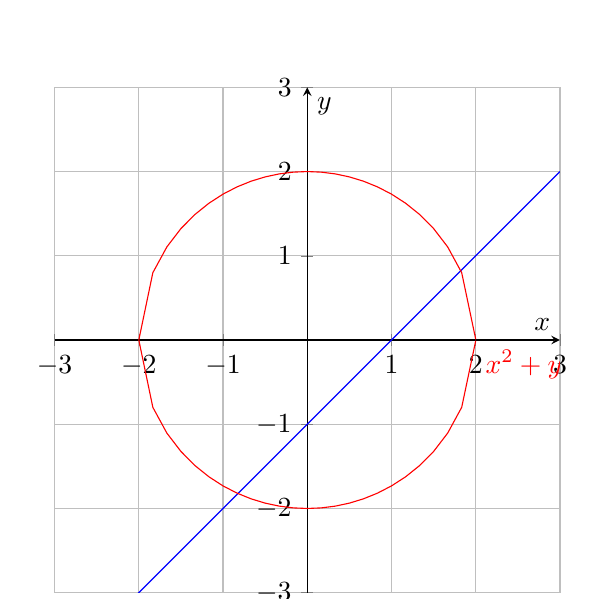
\begin{tikzpicture}
    \begin{axis}[
        axis lines=middle,
        xlabel=$x$,
        ylabel=$y$,
        xmin=-3, xmax=3,
        ymin=-3, ymax=3,
        grid=both,
        width=8cm, height=8cm
    ]
    \addplot[domain=-3:3, blue] {x-1} node[above right] {$y = x - 1$};
    \addplot[domain=-2:2, red] {sqrt(4-x^2)};
    \addplot[domain=-2:2, red] {-sqrt(4-x^2)} node[below right] {$x^2 + y^2 = 4$};
    \end{axis}
\end{tikzpicture}

\section{題庫}
\begin{enumerate}[label=\arabic*.]
    % 計算題 (10)
    \item 求過$(1, -2)$且斜率為$3$的直線方程式。
    \item 將$x^2 + y^2 + 2x - 4y - 4 = 0$化為標準式。
    \item 求直線$2x - 3y + 6 = 0$的斜率與截距。
    \item 求過$(0, 0)$與$(3, 4)$的直線方程式。
    \item 求圓$(x - 1)^2 + (y + 2)^2 = 9$的中心與半徑。
    \item 求點$(2, 1)$到直線$x + y - 3 = 0$的距離。
    \item 判斷直線$y = 2x$與圓$x^2 + y^2 = 1$的關係。
    \item 求過$(1, 1)$且與$x - 2y + 3 = 0$垂直的直線方程式。
    \item 求直線$x = 2$與圓$x^2 + y^2 - 4x = 0$的交點。
    \item 求點$(0, 5)$到直線$3x - 4y + 10 = 0$的距離。
    % 應用題 (10)
    \item 一點沿直線$y = x + 1$移動,求其到$(2, 0)$的最短距離。
    \item 求圓心在$(0, 0)$,過點$(3, 4)$的圓方程式。
    \item 若直線與圓$x^2 + y^2 = 5$相切,求直線斜率(過$(2, 3)$)。
    \item 求點$(1, 1)$到直線$y = -x + 2$的垂足坐標。
    \item 一圓過$(0, 0)$與$(2, 2)$,中心在$x$軸上,求方程式。
    \item 求直線$y = x$與圓$x^2 + y^2 - 2x - 2y + 1 = 0$的交點。
    \item 若直線$kx + y - 2 = 0$與圓$x^2 + y^2 = 2$相交,求$k$範圍。
    \item 求過$(3, 0)$且與圓$x^2 + y^2 = 4$相切的直線方程式。
    \item 一點到直線$2x - y + 1 = 0$的距離為$\sqrt{5}$,求坐標。
    \item 求圓心$(1, 1)$,半徑$2$的圓上斜率為$1$的點。
    % 觀念題 (10)
    \item 證明兩直線垂直時,斜率乘積為$-1$。
    \item 若圓一般式$D^2 + E^2 - 4F < 0$,圖形為何?
    \item 直線與圓相離時,判別式$\Delta$如何?
    \item 說明點到直線距離公式的幾何意義。
    \item 若直線過圓心,交點數為何?
    \item 證明圓的切線垂直於半徑。
    \item 兩直線平行時,法向量有何關係?
    \item 圓心到直線距離等於半徑時,關係為何?
    \item 說明如何用參數式表示直線。
    \item 證明直線$ax + by + c = 0$的法向量為$(a, b)$。
    % 進階題 (10)
    \item 求直線$y = x - 2$與圓$x^2 + y^2 - 4x = 0$的交點。
    \item 若直線與圓$x^2 + y^2 - 2x + 2y - 1 = 0$相切,求直線方程式(過$(0, 0)$)。
    \item 求點$(2, 3)$到直線$x - y + 1 = 0$的垂線方程式。
    \item 求圓$x^2 + y^2 = 1$上距離直線$y = x$最遠的點。
    \item 若直線$3x + 4y + k = 0$與圓$x^2 + y^2 = 5$相交,求$k$範圍。
    \item 求過$(1, 0)$且與圓$x^2 + y^2 - 2x = 0$相切的直線。
    \item 求直線$y = 2x - 1$與圓$x^2 + y^2 - 2y = 0$的弦長。
    \item 若圓心$(0, 0)$,過$(1, 1)$與$(2, 2)$,求方程式。
    \item 求直線$x + y = 1$與圓$x^2 + y^2 - x - y = 0$的交點。
    \item 若直線與圓相切,證明切點到圓心距離等於半徑。
    % 挑戰題 (20)
    \item 求過$(0, 0)$且與圓$x^2 + y^2 - 4x + 2y = 0$相切的直線。
    \item 若直線$y = mx + 1$與圓$x^2 + y^2 = 4$相交,求$m$範圍。
    \item 求點$(3, 4)$到直線$2x + 3y - 6 = 0$的垂足與距離。
    \item 求圓$x^2 + y^2 = 2$與直線$y = x - 1$的交點弦長。
    \item 若直線$ax + by + 1 = 0$與圓$x^2 + y^2 = 1$相切,求$a, b$關係。
    \item 求過$(2, 2)$且與圓$x^2 + y^2 - 2x - 2y + 1 = 0$相交的直線範圍。
    \item 求直線$y = x$與圓$x^2 + y^2 - 4x + 2y = 0$的交點。
    \item 若圓過$(0, 0)$,中心$(a, b)$,半徑$\sqrt{2}$,求方程式範圍。
    \item 求點$(1, 2)$到直線$3x - y + 1 = 0$的垂線與交點。
    \item 若直線與圓$x^2 + y^2 - 2x = 0$相離,求過$(0, 1)$的直線範圍。
    \item 求圓$x^2 + y^2 = 5$上到直線$x + y = 1$距離最大的點。
    \item 若直線$y = kx$與圓$x^2 + y^2 - 4 = 0$相切,求$k$。
    \item 求過$(0, 0)$與$(1, 1)$且與圓$x^2 + y^2 = 1$相交的直線。
    \item 若直線$2x + y + k = 0$與圓$x^2 + y^2 = 2$相切,求$k$。
    \item 求圓$x^2 + y^2 - 2x - 2y + 1 = 0$與直線$x - y = 0$的弦長。
    \item 若直線過$(3, 0)$與圓$x^2 + y^2 = 4$相交,求斜率範圍。
    \item 求點$(0, 0)$到直線$x - 2y + 4 = 0$的垂足與距離。
    \item 若圓心$(1, 1)$,過$(0, 0)$與$(2, 2)$,求方程式。
    \item 求直線$y = 2x - 3$與圓$x^2 + y^2 - 2x = 0$的交點。
    \item 若直線與圓$x^2 + y^2 = 1$相交,求過$(2, 0)$的直線範圍。
\end{enumerate}



\chapter{多項式}

\section{觀念與公式}

\subsection{多項式定義與運算}
多項式是變數與係數的代數式,形式為:
\[
P(x) = a_n x^n + a_{n-1} x^{n-1} + \cdots + a_1 x + a_0, \quad a_n \neq 0
\]
$n$為次數。\\
\textbf{運算}:
\begin{itemize}
    \item 加減:同次項合併。
    \item 乘法:分配律,如$(x + 1)(x - 2) = x^2 - x - 2$。
    \item 除法:$P(x) = Q(x)D(x) + R(x)$,$R(x)$次數低於$D(x)$。
    \item \textbf{綜合除法}:快速除以$(x - a)$,如$P(x) = x^3 - 3x^2 + 2$除以$(x - 1)$:
    \[
    [1, -3, 0, 2] \xrightarrow{1} [1, -2, -2, 0], \quad \text{商} x^2 - 2x - 2, \text{餘數} 0
    \]
\end{itemize}
\textbf{應用}:簡化、找根。\\
\textbf{大學技巧}:綜合除法比長除法高效。

\subsection{餘數定理與因式分解}
\textbf{餘數定理}:$P(x)$除以$(x - a)$,餘數為$P(a)$。若$P(a) = 0$,則$(x - a)$為因式(因式定理)。\\
\textbf{因式分解}:
\begin{itemize}
    \item 提公因式:$2x^2 + 4x = 2x(x + 2)$。
    \item 公式:$x^3 - y^3 = (x - y)(x^2 + xy + y^2)$。
    \item 試根法:用$P(a) = 0$找根,再分解。
\end{itemize}
\textbf{餘數關係延伸}:$P(x)$除以二次式$ax^2 + bx + c$,餘數為$rx + s$,可用待定係數法求解。\\
\textbf{應用}:驗證根、分解多項式。\\
\textbf{大學技巧}:用微分確認根重數,若$P'(a) = 0$,$a$為重根。

\subsection{根與係數關係}
對於$P(x) = a_n x^n + \cdots + a_0$,根$r_1, r_2, \ldots, r_n$滿足(Vieta's公式):
\[
\sum r_i = -\frac{a_{n-1}}{a_n}, \quad \sum r_i r_j = \frac{a_{n-2}}{a_n}, \quad \prod r_i = (-1)^n \frac{a_0}{a_n}
\]
如$x^3 - 6x^2 + 11x - 6$,根和$6$,乘積$6$。\\
\textbf{應用}:求未知係數、驗證根。\\
\textbf{大學技巧}:結合微分分析根的分布。

\subsection{微分與局部特徵}
\textbf{導數}:
\begin{itemize}
    \item $P'(x)$:斜率,$P'(x) = 0$為極值點。
    \item $P''(x)$:凹凸性,$P''(x) > 0$為凹向上。
    \item 重根:$P(a) = P'(a) = 0$,$P''(a) \neq 0$為二重根。
\end{itemize}
\textbf{局部特徵}:單根改變符號,重根不變。\\
\textbf{應用}:極值、單調性。\\
\textbf{大學技巧}:$P^{(k)}(a)$判斷$k$重根。

\subsection{泰勒展開與廣域特徵}
\textbf{泰勒展開}:$P(x)$在$x = a$:
\[
P(x) = P(a) + P'(a)(x - a) + \frac{P''(a)}{2!}(x - a)^2 + \cdots + \frac{P^{(n)}(a)}{n!}(x - a)^n
\]
如$x^3 - x$在$x = 0$,$P(x) = -x + x^3$。\\
\textbf{廣域特徵}:
\begin{itemize}
    \item $n$次多項式有$n$個根(含重根)。
    \item $x \to \pm \infty$,$P(x)$由$a_n x^n$決定。
\end{itemize}
\textbf{應用}:近似、趨勢分析。\\
\textbf{大學技巧}:泰勒展開快速估計局部值。

\subsection{牛頓插值法}
用點$(x_i, y_i)$插值:
\[
P(x) = f(x_0) + f[x_0, x_1](x - x_0) + f[x_0, x_1, x_2](x - x_0)(x - x_1) + \cdots
\]
差商:$f[x_0, x_1] = \frac{f(x_1) - f(x_0)}{x_1 - x_0}$。\\
\textbf{應用}:數據擬合。\\
\textbf{大學技巧}:比拉格朗日插值更高效。

\section{例題解析}

\subsection{例題1:餘數定理}
求$x^3 - 2x^2 + x - 1$除以$(x - 2)$的餘數。\\
\textbf{解}:$P(2) = 8 - 8 + 2 - 1 = 1$。綜合除法驗證:
\[
[1, -2, 1, -1] \xrightarrow{2} [1, 0, 1, 1], \quad \text{餘數} 1
\]
\textbf{大學技巧}:餘數定理直接得出。

\subsection{例題2:根與係數}
若$x^3 - kx^2 + 5x - 2 = 0$的根和為$3$,求$k$。\\
\textbf{解}:$\sum r_i = \frac{k}{1} = 3$,$k = 3$。\\
\textbf{大學技巧}:試根$P(1) = 2$,調整驗證。

\subsection{例題3:泰勒展開}
求$x^3 - 3x + 1$在$x = 1$的泰勒展開(至二階)。\\
\textbf{解}:$P(1) = -1$,$P'(x) = 3x^2 - 3$,$P'(1) = 0$,$P''(x) = 6x$,$P''(1) = 6$:
\[
P(x) = -1 + 0(x - 1) + 3(x - 1)^2
\]
\textbf{大學技巧}:全展開等於原式。

\subsection{例題4:牛頓插值}
用點$(0, 1), (1, 0), (2, 3)$插值。\\
\textbf{解}:差商:
\[
f[0, 1] = -1, \quad f[1, 2] = 3, \quad f[0, 1, 2] = 2
\]
\[
P(x) = 1 - x + 2x(x - 1) = 2x^2 - 3x + 1
\]
\textbf{大學技巧}:驗證點值吻合。

\section{圖形展示}
$x^3 - 3x + 1$:
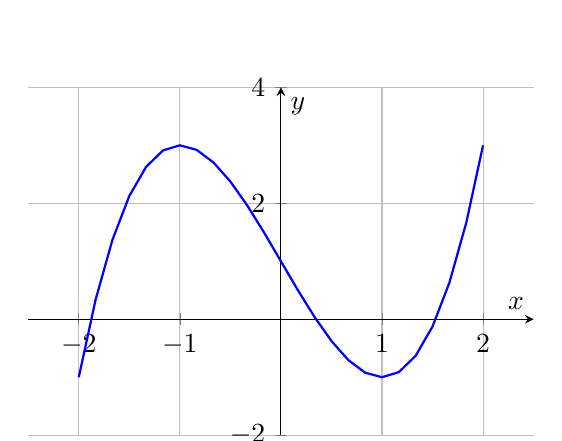
\begin{tikzpicture}
    \begin{axis}[
        axis lines=middle,
        xlabel=$x$,
        ylabel=$y$,
        xmin=-2.5, xmax=2.5,
        ymin=-2, ymax=4,
        grid=both,
        width=8cm, height=6cm
    ]
    \addplot[domain=-2:2, blue, thick] {x^3 - 3*x + 1};
    \end{axis}
\end{tikzpicture}

\section{題庫}
\begin{enumerate}[label=\arabic*.]
    % 計算題 (10)
    \item 計算$(x + 1)(x^2 - 2x + 1)$。
    \item 分解$x^3 - 8$。
    \item 求$x^3 - 3x^2 + 2x - 1$除以$(x - 1)$的餘數。
    \item 分解$x^4 - 16$。
    \item 若$P(x) = x^3 - 2x + 1$,求$P(2)$。
    \item 用綜合除法求$x^3 - 4x^2 + 5x - 2$除以$(x - 2)$的商。
    \item 分解$x^2 - 4x + 4$。
    \item 求$x^3 - x + 1$在$x = 0$的泰勒展開(至二階)。
    \item 若$P(x) = x^3 + x^2 - x - 1$,求$P(-1)$。
    \item 分解$x^3 + 27$。
    % 應用題 (10)
    \item 求$x^3 - 3x^2 + 3x - 1$的實根與重數。
    \item 若$P(x) = x^3 - 5x^2 + kx - 2$根和為$5$,求$k$。
    \item 求$x^3 - 2x + 1$在$[0, 1]$的最小值。
    \item 用點$(0, 0), (1, 1), (2, 0)$插值多項式。
    \item 求$x^4 - 4x^2 + 3$的極值點。
    \item 若$P(x) = x^3 - 6x^2 + 11x - 6$,求根的乘積。
    \item 求$x^3 - x^2 + x - 1$在$[-1, 1]$的最大值。
    \item 若$P(x) = x^3 + 2x^2 - 5x - 6$,求單調區間。
    \item 求$x^3 - 3x + 2$的廣域趨勢。
    \item 若$P(x) = x^4 - 2x^2 + 1$,求$P''(x)$的根。
    % 觀念題 (10)
    \item 證明餘數定理:$P(x) = (x - a)Q(x) + P(a)$。
    \item 若$P(x)$有二重根,$P'(a)$如何?
    \item 說明根與係數關係的應用。
    \item 若$P(x)$為三次多項式,實根數可能為何?
    \item 證明泰勒展開對於多項式的有限項。
    \item 說明綜合除法如何找根。
    \item 若$P(x)$趨向負無窮,$a_n$如何?
    \item 證明$x^3 - x + 1$至多1實根。
    \item 說明牛頓插值如何保證唯一。
    \item 若$P(x)$除以$(x^2 + 1)$,餘數形式為何?
    % 進階題 (10)
    \item 求$x^3 - 4x^2 + 5x - 2$的所有實根。
    \item 若$P(x) = x^4 - 5x^2 + 4$,求極值。
    \item 求$x^3 - 6x^2 + 9x - 4$的局部特徵。
    \item 用綜合除法求$x^3 - 2x^2 + x - 1$除以$(x - 1)$的商。
    \item 求$x^3 + 2x^2 - x - 2$在$x = 1$的泰勒展開(至一階)。
    \item 若$P(x) = x^3 - 3x^2 + 2x - 1$,求$P'(x)$的根。
    \item 求$x^4 - 2x^3 + x^2 - 2x + 1$的實根數。
    \item 若$P(x) = x^3 - x^2 - x + 1$,求廣域特徵。
    \item 用點$(0, 1), (1, 2), (2, 5)$插值多項式。
    \item 求$x^3 - 5x^2 + 8x - 4$的根與重數。
    % 挑戰題 (20)
    \item 若$P(x) = x^4 - 4x + 3$,求所有實根與極值。
    \item 求$x^3 - 3x^2 + 3x - 1$在$x = 1$的泰勒展開(至三階)。
    \item 若$P(x) = x^5 - 5x + 4$,求實根數。
    \item 求$x^3 - 4x^2 + 5x - 2$的餘數關係(除以$x - 3$)。
    \item 若$P(x) = x^4 - 2x^2 - 3$,求極值與根。
    \item 求$x^3 + 2x^2 - 5x - 6$的所有實根。
    \item 用綜合除法分解$x^4 - 3x^3 + 2x^2 - x + 1$除以$(x - 1)$。
    \item 若$P(x) = x^3 - x^2 - x + 1$,求$x \in [-1, 1]$的最小值。
    \item 求$x^3 - 6x^2 + 11x - 6$的根與係數關係。
    \item 用點$(0, 0), (1, 1), (2, 4)$插值多項式。
    \item 若$P(x) = x^4 - 2x^3 + x^2 - 2x + 1$,求極值。
    \item 求$x^3 - 3x^2 + 2x - 1$在$[0, 1]$的最大值。
    \item 若$P(x) = x^3 + x^2 - 2x - 2$,求單調區間。
    \item 求$x^4 - 4x^2 + 3$在$[0, 2]$的最大值。
    \item 若$P(x) = x^3 - 2x^2 - 5x + 6$,求$P''(x)$的根。
    \item 求$x^3 - 5x^2 + 8x - 4$在$x = 1$的泰勒展開(至二階)。
    \item 若$P(x) = x^4 - x^2 + 1$,求廣域特徵。
    \item 求$x^3 + 3x^2 - 4x - 12$的所有實根。
    \item 用綜合除法求$x^3 - 4x^2 + 3x + 1$除以$(x - 2)$的商。
    \item 若$P(x) = x^5 - x^3 + x - 1$,求$x \in [0, 1]$的最小值。
\end{enumerate}


\chapter{數列與級數}

\section{觀念與公式}

\subsection{數列的基本概念}
數列是有序的數字序列,如$1, 4, 7, 10, \ldots$。\\
\textbf{表示法}:
\begin{itemize}
    \item 通項:$a_n$,如$a_n = 3n - 2$。
    \item 遞推:$a_n = a_{n-1} + d$,需給初值。
\end{itemize}
\textbf{類型}:等差、等比、費氏數列。\\
\textbf{應用}:描述規律變化。\\
\textbf{大學技巧}:用生成函數分析遞推數列。

\subsection{等差數列}
每項與前項差為常數$d$(公差)。\\
\textbf{公式}:
\begin{itemize}
    \item 通項:$a_n = a_1 + (n-1)d$。
    \item 總和:$S_n = \frac{n}{2} (a_1 + a_n)$ 或 $S_n = \frac{n}{2} [2a_1 + (n-1)d]$。
\end{itemize}
\textbf{性質}:線性增長。\\
\textbf{應用}:均勻增加問題。\\
\textbf{大學技巧}:用數學歸納法證總和公式。

\subsection{等比數列}
每項與前項比為常數$r$(公比)。\\
\textbf{公式}:
\begin{itemize}
    \item 通項:$a_n = a_1 r^{n-1}$。
    \item 總和:$S_n = a_1 \frac{1 - r^n}{1 - r}$($r \neq 1$)。
    \item 無限級數:若$|r| < 1$,$S_\infty = \frac{a_1}{1 - r}$。
\end{itemize}
\textbf{性質}:指數增長或衰減。\\
\textbf{應用}:利息、折舊。\\
\textbf{大學技巧}:判斷級數收斂性。

\subsection{級數}
數列項的和$S_n = a_1 + a_2 + \cdots + a_n$。\\
\textbf{類型}:
\begin{itemize}
    \item 有限級數:固定項數。
    \item 無限級數:需判斷收斂。
\end{itemize}
\textbf{應用}:累積總量。\\
\textbf{大學技巧}:泰勒級數近似函數。

\subsection{數學歸納法}
證明數列性質:
\begin{enumerate}
    \item 基礎步:驗證$n = 1$。
    \item 歸納步:假設$n = k$成立,證$n = k+1$。
\end{enumerate}
\textbf{應用}:證總和公式。\\
\textbf{大學技巧}:證複雜遞推關係。

\section{例題解析}

\subsection{例題1:等差數列(計算題)}
一等差數列首項$3$,公差$2$,求第10項與前10項和。\\
\textbf{解}:通項$a_n = 3 + (n-1) \cdot 2$,$a_{10} = 3 + 9 \cdot 2 = 21$。\\
總和$S_{10} = \frac{10}{2} (3 + 21) = 5 \cdot 24 = 120$。\\
\textbf{大學技巧}:驗證$a_{10} - a_9 = 2$。

\subsection{例題2:等比數列(應用題)}
一物品價值1000元,每年折舊20\%,求第5年價值與5年總價值。\\
\textbf{解}:$a_n = 1000 \cdot (0.8)^{n-1}$,$a_5 = 1000 \cdot (0.8)^4 = 409.6$元。\\
$S_5 = 1000 \frac{1 - (0.8)^5}{1 - 0.8} = 1000 \cdot \frac{1 - 0.32768}{0.2} = 3361.6$元。\\
\textbf{大學技巧}:無限折舊$S_\infty = \frac{1000}{0.2} = 5000$元。

\subsection{例題3:遞推數列(觀念題)}
費氏數列$a_1 = 1, a_2 = 1, a_n = a_{n-1} + a_{n-2}$,求$a_6$。\\
\textbf{解}:$a_3 = 2, a_4 = 3, a_5 = 5, a_6 = 8$。\\
\textbf{大學技巧}:黃金比例近似$a_n \approx \frac{\phi^n}{\sqrt{5}}$,$\phi = \frac{1 + \sqrt{5}}{2}$。

\subsection{例題4:數學歸納法}
證$S_n = \frac{n}{2} [2a_1 + (n-1)d]$。\\
\textbf{解}:$n = 1$,$S_1 = a_1$成立。假設$n = k$成立,$n = k+1$:
\[
S_{k+1} = S_k + a_{k+1} = \frac{k}{2} [2a_1 + (k-1)d] + [a_1 + kd] = \frac{k+1}{2} [2a_1 + kd]
\]
成立。\\
\textbf{大學技巧}:用連續和推導。

\section{圖形展示}
等比數列$a_n = 2 \cdot (0.5)^{n-1}$:
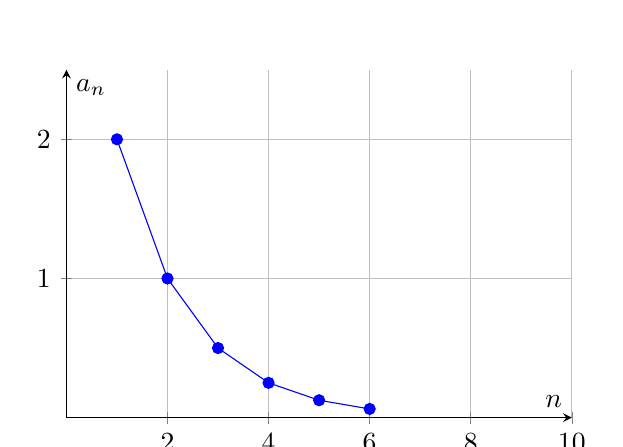
\begin{tikzpicture}
    \begin{axis}[
        axis lines=middle,
        xlabel=$n$,
        ylabel=$a_n$,
        xmin=0, xmax=10,
        ymin=0, ymax=2.5,
        grid=both,
        width=8cm, height=6cm
    ]
    \addplot[mark=*, blue] coordinates {(1,2) (2,1) (3,0.5) (4,0.25) (5,0.125) (6,0.0625)};
    \end{axis}
\end{tikzpicture}

\section{題庫}
\begin{enumerate}[label=\arabic*.]
    % 計算題 (10)
    \item 求等差數列$a_1 = 5, d = 3$的$a_{10}$。
    \item 求等比數列$a_1 = 2, r = 2$的$S_5$。
    \item 若$a_n = 4n - 1$,求$S_{10}$。
    \item 求等差數列$a_1 = 1, a_5 = 9$的$d$。
    \item 求等比數列$a_1 = 3, r = \frac{1}{2}$的$a_6$。
    \item 若$a_1 = 2, d = -1$,求$S_{20}$。
    \item 求$a_n = a_{n-1} + 3, a_1 = 1$的$a_8$。
    \item 求等比數列$a_1 = 1, r = -2$的$S_4$。
    \item 若$a_1 = 10, d = 2$,求$a_{15}$。
    \item 求等比數列$a_1 = 4, r = 0.5$的$S_\infty$。
    % 應用題 (10)
    \item 一存款首年1000元,每年增200元,求第10年總額。
    \item 一球從10公尺落下,每次反彈前高0.8倍,求總距離。
    \item 若$a_1 = 1, a_n = 2a_{n-1}$,求$S_6$。
    \item 一數列$a_1 = 3, d = 4$,求第幾項為$35$。
    \item 一物品首年值5000元,年折舊10\%,求5年總值。
    \item 若$S_n = 3n^2 + 1$,求$a_n$。
    \item 一等差數列$a_1 = 2, S_{10} = 110$,求$d$。
    \item 一等比數列$a_1 = 2, S_5 = 62$,求$r$。
    \item 若$a_1 = 1, a_n = a_{n-1} + n$,求$a_5$。
    \item 一數列$a_1 = 5, r = \frac{1}{3}$,求$S_\infty$。
    % 觀念題 (10)
    \item 證等差數列$S_n = \frac{n}{2} (a_1 + a_n)$。
    \item 等比數列$|r| > 1$時,$S_\infty$是否存在?
    \item 說明數學歸納法的步驟。
    \item 若$a_n = a_{n-1} + 2$,求通項。
    \item 證$S_n = a_1 \frac{1 - r^n}{1 - r}$。
    \item 等差數列總和公式有幾種形式?
    \item 若$a_n = 2^n$,求$S_n$。
    \item 說明費氏數列的遞推關係。
    \item 若$S_n = n(n+1)$,求$a_n$。
    \item 等比數列收斂條件為何?
    % 進階題 (10)
    \item 求$a_1 = 1, d = 3$,$S_n = 100$的$n$。
    \item 若$a_1 = 2, r = 3$,求$a_5$與$S_5$。
    \item 求$a_n = a_{n-1} + a_{n-2}, a_1 = 1, a_2 = 1$的$a_7$。
    \item 若$S_n = 2^n - 1$,求$a_n$。
    \item 求$a_1 = 4, d = -2$,$a_n = -10$的$n$。
    \item 若$a_1 = 1, r = \frac{1}{2}$,求$n$使$S_n > 1.9$。
    \item 求$a_1 = 3, d = 5$,$S_{10}$。
    \item 若$a_1 = 2, r = -1$,求$S_{100}$。
    \item 求$a_n = 3n^2 - 1$的$S_5$。
    \item 若$a_1 = 1, a_n = 3a_{n-1}$,求$a_6$。
    % 挑戰題 (20)
    \item 一等差數列$a_1 = 2, a_{10} = 20$,求$S_{10}$。
    \item 若$a_1 = 1, r = 2$,求$n$使$a_n > 1000$。
    \item 求$a_1 = 5, d = -3$,$S_n = -20$的$n$。
    \item 若$a_1 = 3, r = \frac{1}{2}$,求$n$使$S_n > 5.9$。
    \item 求$a_n = a_{n-1} + 2n, a_1 = 1$的$a_5$。
    \item 若$S_n = \frac{n(n+1)(2n+1)}{6}$,求$a_n$。
    \item 求$a_1 = 1, r = -2$,$S_6$。
    \item 若$a_1 = 4, d = 2$,求$n$使$S_n > 100$。
    \item 求$a_n = 2^n$的$S_{10}$。
    \item 若$a_1 = 2, a_n = a_{n-1} + 3$,求$S_8$。
    \item 求$a_1 = 3, r = 0.5$,$S_n = 5.25$的$n$。
    \item 若$a_1 = 1, d = 4$,求$a_{20}$與$S_{20}$。
    \item 求$a_n = n^2$的$S_5$。
    \item 若$a_1 = 5, r = \frac{2}{3}$,求$S_\infty$。
    \item 求$a_1 = 2, d = -1$,$S_{15}$。
    \item 若$a_1 = 1, a_n = a_{n-1} + a_{n-2}$,求$a_8$。
    \item 求$a_1 = 10, r = 0.9$,$S_{10}$。
    \item 若$a_1 = 3, d = 2$,求$n$使$a_n = 45$。
    \item 求$a_n = 3n - 2$的$S_{10}$。
    \item 若$a_1 = 1, r = 3$,求$n$使$S_n > 1000$。
\end{enumerate}



\chapter{指數與對數}
% src/chapter5.tex


\section{觀念與公式}

\subsection{指數的基本概念}
指數表示連乘,$a^n = a \cdot a \cdots a$($n$次),$a > 0$。\\
\textbf{指數律}:
\begin{itemize}
    \item $a^m \cdot a^n = a^{m+n}$
    \item $\frac{a^m}{a^n} = a^{m-n}$
    \item $(a^m)^n = a^{mn}$
    \item $a^{-n} = \frac{1}{a^n}$,$a^{\frac{m}{n}} = \sqrt[n]{a^m}$
\end{itemize}
\textbf{應用}:簡化運算。\\
\textbf{大學技巧}:指數的連續性,$a^x = e^{x \ln a}$。

\subsection{指數函數}
定義:$f(x) = a^x$,$a > 0$且$a \neq 1$。\\
\textbf{性質}:
\begin{itemize}
    \item $a > 1$:單調遞增,$x \to \infty$時$f(x) \to \infty$。
    \item $0 < a < 1$:單調遞減,$x \to \infty$時$f(x) \to 0$。
\end{itemize}
\textbf{應用}:增長模型。\\
\textbf{大學技巧}:微分$\frac{d}{dx} a^x = a^x \ln a$。

\subsection{對數的基本概念}
若$a^x = b$,則$\log_a b = x$,$a > 0$且$a \neq 1$。\\
\textbf{對數律}:
\begin{itemize}
    \item $\log_a (mn) = \log_a m + \log_a n$
    \item $\log_a \left(\frac{m}{n}\right) = \log_a m - \log_a n$
    \item $\log_a (m^n) = n \log_a m$
    \item 換底公式:$\log_a b = \frac{\log_c b}{\log_c a}$
\end{itemize}
\textbf{應用}:化簡複雜運算。\\
\textbf{大學技巧}:自然對數$\ln x$,底$e \approx 2.718$。

\subsection{對數函數}
定義:$f(x) = \log_a x$,$x > 0$。\\
\textbf{性質}:
\begin{itemize}
    \item $a > 1$:單調遞增,過$(1, 0)$。
    \item $0 < a < 1$:單調遞減。
\end{itemize}
\textbf{應用}:壓縮數據。\\
\textbf{大學技巧}:微分$\frac{d}{dx} \log_a x = \frac{1}{x \ln a}$。

\subsection{指數與對數的互逆}
\begin{itemize}
    \item $a^{\log_a x} = x$($x > 0$)
    \item $\log_a (a^x) = x$
\end{itemize}
\textbf{應用}:解方程。\\
\textbf{大學技巧}:泰勒展開,如$\ln(1+x) \approx x - \frac{x^2}{2}$。

\section{例題解析}

\subsection{例題1:指數運算(計算題)}
化簡$2^3 \cdot 2^{-1} \cdot 4^2$。\\
\textbf{解}:$4 = 2^2$,則:
\[
2^3 \cdot 2^{-1} \cdot (2^2)^2 = 2^3 \cdot 2^{-1} \cdot 2^4 = 2^{3-1+4} = 2^6 = 64
\]
\textbf{大學技巧}:用$a^x = e^{x \ln a}$驗算。

\subsection{例題2:對數運算(計算題)}
化簡$\log_2 8 + \log_2 \left(\frac{1}{4}\right)$。\\
\textbf{解}:
\[
\log_2 8 + \log_2 \left(\frac{1}{4}\right) = \log_2 (8 \cdot \frac{1}{4}) = \log_2 2 = 1
\]
\textbf{大學技巧}:換底公式驗證。

\subsection{例題3:解方程(應用題)}
解$3^{x+1} = 27$。\\
\textbf{解}:$27 = 3^3$,則:
\[
3^{x+1} = 3^3 \implies x + 1 = 3 \implies x = 2
\]
或取對數:$\log_3 (3^{x+1}) = \log_3 27$,$x + 1 = 3$。\\
\textbf{大學技巧}:用$\ln$解,$\ln (3^{x+1}) = \ln 27$。

\subsection{例題4:應用問題}
一物質每小時衰減20\%,求半衰期。\\
\textbf{解}:設初量$Q_0$,$Q(t) = Q_0 (0.8)^t$,半衰期時$Q(t) = \frac{Q_0}{2}$:
\[
(0.8)^t = 0.5 \implies t \log 0.8 = \log 0.5 \implies t = \frac{\log 0.5}{\log 0.8} \approx 3.1 \text{小時}
\]
\textbf{大學技巧}:用$\ln$,$t = \frac{\ln 0.5}{\ln 0.8}$。

\section{圖形展示}
指數函數$y = 2^x$與對數函數$y = \log_2 x$:
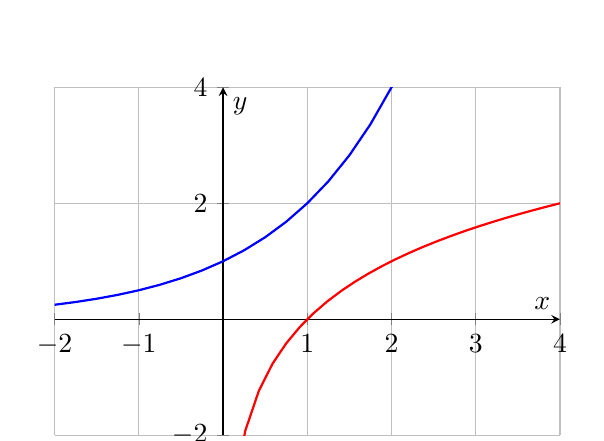
\begin{tikzpicture}
    \begin{axis}[
        axis lines=middle,
        xlabel=$x$,
        ylabel=$y$,
        xmin=-2, xmax=4,
        ymin=-2, ymax=4,
        grid=both,
        width=8cm, height=6cm
    ]
    \addplot[domain=-2:4, blue, thick] {2^x} node[above] {$y = 2^x$};
    \addplot[domain=0.1:4, red, thick] {log2(x)} node[below right] {$y = \log_2 x$};
    \end{axis}
\end{tikzpicture}

\section{題庫}
\begin{enumerate}[label=\arabic*.]
    % 計算題 (10)
    \item 化簡$3^2 \cdot 3^{-3} \cdot 9$。
    \item 計算$\log_4 16$。
    \item 化簡$\log_5 25 + \log_5 125$。
    \item 求$2^{-2} \cdot 8$。
    \item 計算$\log_3 81$。
    \item 化簡$4^{\frac{3}{2}}$。
    \item 求$\log_2 \left(\frac{1}{8}\right)$。
    \item 化簡$10^2 \cdot 10^{-1}$。
    \item 計算$\log_{10} 1000$。
    \item 求$5^0 \cdot 5^3$。
    % 應用題 (10)
    \item 解$2^x = 16$。
    \item 一存款1000元,年利率5\%複利,求5年後金額。
    \item 解$\log_3 (x - 1) = 2$。
    \item 一物質半衰期10小時,求每小時衰減率。
    \item 解$4^{x-1} = 64$。
    \item 若$\log_a 8 = 3$,求$a$。
    \item 一人口每年增長2\%,幾年後翻倍。
    \item 解$\log_2 x + \log_2 (x - 1) = 1$。
    \item 若$pH = -\log_{10} [H^+]$,$[H^+] = 10^{-7}$,求$pH$。
    \item 解$5^{2x} = 125$。
    % 觀念題 (10)
    \item 證$a^{\log_a x} = x$。
    \item 說明指數函數的單調性。
    \item 證$\log_a (mn) = \log_a m + \log_a n$。
    \item 若$a^x = a^y$,則$x, y$關係為何?
    \item 說明對數函數的定義域。
    \item 證$\log_a \left(\frac{m}{n}\right) = \log_a m - \log_a n$。
    \item 若$\log_a b = c$,則$b$如何表示?
    \item 說明換底公式的推導。
    \item 指數函數與對數函數的圖形關係為何?
    \item 若$a > 1$,$\log_a x$的範圍為何?
    % 進階題 (10)
    \item 解$2^{x+1} = 3$(近似值)。
    \item 若$\log_2 x = 3 + \log_2 (x-1)$,求$x$。
    \item 求$3^x$在$x = 2$的泰勒展開(至一階)。
    \item 解$10^{2x-1} = 100$。
    \item 若$\log_a 5 + \log_a 2 = 1$,求$a$。
    \item 求一物質衰減率0.1/小時,半衰期。
    \item 解$2^x + 2^{-x} = 5$。
    \item 若$\log_3 (x^2) = 4$,求$x$。
    \item 解$\log_5 (x+1) - \log_5 (x-1) = 2$。
    \item 若$y = \ln x$,求$x = 1$時斜率。
    % 挑戰題 (20)
    \item 解$3^{x+2} = 5^{x-1}$(近似值)。
    \item 若$\log_2 (x+1) + \log_2 (x-1) = 3$,求$x$。
    \item 求$\ln (1+x)$在$x = 0$的泰勒展開(至三階)。
    \item 解$4^x - 2^x = 3$。
    \item 若$\log_a 3 = 0.5$,求$a$。
    \item 一物質每小時衰減至前值的$\frac{1}{3}$,求半衰期。
    \item 解$2^{2x} - 5 \cdot 2^x + 4 = 0$。
    \item 若$\log_2 (x+2) = 2 + \log_2 x$,求$x$。
    \item 解$\log_3 (x-2) + \log_3 (x+2) = 2$。
    \item 若$y = 2^x$,求$x = 0$時斜率。
    \item 解$5^x = 2^{x+1}$(近似值)。
    \item 若$\log_{10} x = 2 - \log_{10} (x-1)$,求$x$。
    \item 求$e^x$在$x = 0$的泰勒展開(至二階)。
    \item 解$3^{x-1} + 3^{1-x} = 10$。
    \item 若$\log_a 4 = 2 \log_a 2$,求$a$。
    \item 一人口首年1000,每年增長10\%,求10年後人口。
    \item 解$2^x - 2^{-x} = 1$。
    \item 若$\log_5 (x^2 - 1) = 2$,求$x$。
    \item 解$\log_2 (x+3) - \log_2 (x-1) = 3$。
    \item 若$y = \log_3 x$,求$x = 9$時斜率。
\end{enumerate}



\chapter{排列組合}

\section{觀念與公式}

\subsection{基本概念}
排列與組合處理選擇與排列問題。\\
\textbf{定義}:
\begin{itemize}
    \item 排列:$P(n, k) = \frac{n!}{(n-k)!}$,從n個取k個有序排列。
    \item 組合:$\binom{n}{k} = \frac{n!}{k!(n-k)!}$,從n個取k個無序組合。
    \item 階乘:$n! = n \cdot (n-1) \cdots 1$,$0! = 1$。
\end{itemize}
\textbf{應用}:計數問題。\\
\textbf{大學技巧}:用生成函數求解。

\subsection{排列的應用}
\textbf{公式}:
\begin{itemize}
    \item 全排列:$n!$。
    \item 環狀排列:$(n-1)!$。
    \item 有重複排列:$\frac{n!}{n_1! n_2! \cdots n_k!}$。
    \item \textbf{Hn取k}:從n個不同物取k個(可重複),$n^k$。
\end{itemize}
\textbf{應用}:排隊、密碼。\\
\textbf{大學技巧}:容斥原理處理限制。

\subsection{組合的應用}
\textbf{公式}:
\begin{itemize}
    \item 基本組合:$\binom{n}{k}$。
    \item 二項式定理:$(a + b)^n = \sum_{k=0}^n \binom{n}{k} a^{n-k} b^k$。
    \item 性質:$\binom{n}{k} = \binom{n}{n-k}$,帕斯卡公式$\binom{n}{k} + \binom{n}{k-1} = \binom{n+1}{k}$。
\end{itemize}
\textbf{應用}:選物、分組。\\
\textbf{大學技巧}:組合恆等式。

\subsection{卡特蘭數}
定義:$C_n = \frac{1}{n+1} \binom{2n}{n}$。\\
\textbf{應用}:
\begin{itemize}
    \item 括號配對:$C_3 = 5$。
    \item 不越界路徑:從$(0,0)$到$(n,n)$。
\end{itemize}
\textbf{值}:$C_0 = 1, C_1 = 1, C_2 = 2, C_3 = 5, C_4 = 14$。\\
\textbf{大學技巧}:遞推$C_n = \sum_{i=0}^{n-1} C_i C_{n-1-i}$。

\section{例題解析}

\subsection{例題1:條件排列}
5人排隊,A, B相鄰,求方法數。\\
\textbf{解}:視A, B為一組,則4個單位(AB, 3人),全排列$4! = 24$,AB內部2種排法,總數$24 \cdot 2 = 48$。\\
\textbf{大學技巧}:容斥法驗證。

\subsection{例題2:分組應用}
從6人選3人分給A組,餘下給B組,求方法數。\\
\textbf{解}:選3人給A組,$\binom{6}{3} = 20$,餘下自動分B組,總數$20$。\\
\textbf{大學技巧}:考慮組內排列。

\subsection{例題3:卡特蘭數應用}
求4個節點的二叉樹數量。\\
\textbf{解}:二叉樹數為$C_4 = \frac{1}{5} \binom{8}{4} = \frac{70}{5} = 14$。\\
\textbf{大學技巧}:用路徑計數。

\subsection{例題4:重複排列應用}
從3種顏色選4個塗4格(可重複),求方法數。\\
\textbf{解}:$H(3, 4) = 3^4 = 81$。\\
\textbf{大學技巧}:生成函數$(x_1 + x_2 + x_3)^4$。

\subsection{例題5:二項式應用}
求$(3x - 2)^5$的$x^3$項係數。\\
\textbf{解}:$(3x)^{5-k} (-2)^k$,$5-k=3$,$k=2$:
\[
\binom{5}{2} \cdot 3^3 \cdot (-2)^2 = 10 \cdot 27 \cdot 4 = 1080
\]
\textbf{大學技巧}:用係數提取。



\section{題庫}
\begin{enumerate}[label=\arabic*.]
    % 計算題 (10)
    \item 求$P(5, 3)$。
    \item 求$\binom{6}{2}$。
    \item 求$4!$。
    \item 用A, A, B排3位序列,求方法數。
    \item 求$(x + 2)^4$的$x^2$項係數。
    \item 求$P(7, 2)$。
    \item 求$\binom{8}{3}$。
    \item 用1, 1, 2排3位序列,求方法數。
    \item 從4人排成一圈,求方法數。
    \item 求$\binom{5}{4}$。
    % 應用題 (20)
    \item 5人排隊,A, B相鄰,求方法數。
    \item 從6人選3人組成委員會,A必選,求方法數。
    \item 4人圍圓桌,A, B不相鄰,求方法數。
    \item 從8本書選4本分給2人,每人2本,求方法數。
    \item 用0, 1組成5位數(可重複),至少1個0,求方法數。
    \item 6個不同球分3堆(可空),求方法數。
    \item 從5男3女選4人,至少1女,求方法數。
    \item 求$(2x - 1)^6$的$x^4$項係數。
    \item 5人排隊,A在B前,求方法數。
    \item 從7個數字選3個,至少1奇數,求方法數。
    \item 6人圍圓桌,A, B, C順時針連續,求方法數。
    \item 用A, B, C排4位序列,至少2個A,求方法數。
    \item 從10人選5人,至少2人為特定組(4人),求方法數。
    \item 5個不同物分2堆(不可空),求方法數。
    \item 從4種顏色選3格塗色(可重複),求方法數。
    \item 7人排隊,A, B相鄰且C在D前,求方法數。
    \item 求$C_4$(卡特蘭數)。
    \item 從6個數字選3個排成3位數,至少1個5,求方法數。
    \item 8人選4人分2組,每組2人,求方法數。
    \item 從5人選3人排隊,A, B不相鄰,求方法數。
    % 觀念題 (10)
    \item 證$\binom{n}{k} = \binom{n}{n-k}$。
    \item 說明環狀排列的公式推導。
    \item 證帕斯卡恆等式。
    \item 若有重複物,排列公式為何?
    \item 說明二項式定理如何求係數。
    \item 卡特蘭數如何應用於路徑計數?
    \item 若從n個取k個可重複,方法數為何?
    \item 證$P(n, k) = n \cdot (n-1) \cdots (n-k+1)$。
    \item 說明組合與排列的區別。
    \item 二項式展開的總係數和為何?
    % 進階題 (10)
    \item 從6人選3人排隊,A必須在首位,求方法數。
    \item 求$(3x + 2)^5$的$x^3$項係數。
    \item 用A, A, B, C, D排5位序列,求方法數。
    \item 求$C_5$(卡特蘭數)。
    \item 從8人選4人,A, B必選,求方法數。
    \item 若$(x - 3)^7$的$x^5$項為$kx^5$,求$k$。
    \item 6人排隊,A, B, C中至少2人相鄰,求方法數。
    \item 從5種數字選4個(可重複),至少1個1,求方法數。
    \item 7人圍圓桌,A, B相鄰且C不在D旁,求方法數。
    \item 從9人選5人,至少3人為特定組(4人),求方法數。
    % 挑戰題 (10)
    \item 6人排隊,A, B相鄰且C, D不相鄰,求方法數。
    \item 求$(2x - y)^6$的$x^4 y^2$項係數。
    \item 5個不同球分3堆,至少1堆空,求方法數。
    \item 用A, A, A, B, B, C排6位序列,求方法數。
    \item 從7男3女選5人,至少2男2女,求方法數。
    \item 8人圍圓桌,A, B, C順時針連續且D不在E旁,求方法數。
    \item 若$(x + 2y)^8$的$x^4 y^4$項為$kx^4 y^4$,求$k$。
    \item 從6個數字選3個,至少1個5且1個7,求方法數。
    \item 5人排隊,A在B前且C在D前,求方法數。
    \item 從10本書選5本分3人,每人至少1本,求方法數。
\end{enumerate}



\chapter{數據分析}
\section{觀念與公式}

\subsection{數據的表示與整理}
數據分析從整理開始。\\
\textbf{方法}:
\begin{itemize}
    \item 頻率表、分組頻率表。
    \item 圖表:直方圖、折線圖、圓餅圖、莖葉圖、箱形圖(五數概要:$Q_1, Q_2, Q_3, \text{最小值}, \text{最大值}$)。
\end{itemize}
\textbf{應用}:視覺化數據。\\
\textbf{大學技巧}:用Python繪圖。

\subsection{中心量數}
衡量數據集中趨勢。\\
\textbf{公式}:
\begin{itemize}
    \item 平均數:$\bar{x} = \frac{\sum x_i}{n}$。
    \item 中位數:排序後中間值。
    \item 眾數:出現次數最多值。
\end{itemize}
\textbf{應用}:比較數據特性。\\
\textbf{大學技巧}:加權平均。

\subsection{離散程度}
衡量數據分散性。\\
\textbf{公式}:
\begin{itemize}
    \item 全距:最大值 - 最小值。
    \item 四分位距:$IQR = Q_3 - Q_1$。
    \item 變異數:$s^2 = \frac{\sum (x_i - \bar{x})^2}{n}$(樣本用$n-1$)。
    \item 標準差:$s = \sqrt{s^2}$。
\end{itemize}
\textbf{應用}:數據穩定性。\\
\textbf{大學技巧}:常態分佈68-95-99.7規則。

\subsection{數據分佈}
描述數據形狀。\\
\textbf{類型}:
\begin{itemize}
    \item 對稱分佈:平均數 $\approx$ 中位數。
    \item 偏態分佈:右偏(平均數 > 中位數)、左偏(平均數 < 中位數)。
    \item 常態分佈:鐘形曲線。
\end{itemize}
\textbf{應用}:判斷特性。\\
\textbf{大學技巧}:標準化$z = \frac{x - \mu}{\sigma}$。

\subsection{雙變量數據分析}
探索兩變量關係。\\
\textbf{方法}:
\begin{itemize}
    \item 散佈圖:觀察數據點分佈。
    \item 相關係數(皮爾森):$r = \frac{\sum (x_i - \bar{x})(y_i - \bar{y})}{\sqrt{\sum (x_i - \bar{x})^2 \sum (y_i - \bar{y})^2}}$,範圍$-1 \leq r \leq 1$。
    \item 迴歸直線:$y = ax + b$,斜率$a = \frac{\sum (x_i - \bar{x})(y_i - \bar{y})}{\sum (x_i - \bar{x})^2}$。
\end{itemize}
\textbf{性質}:
\begin{itemize}
    \item $r > 0$:正相關,$r < 0$:負相關,$r \approx 0$:無線性相關。
    \item $|r|$接近1表示強相關,接近0表示弱相關。
\end{itemize}
\textbf{應用}:預測與解釋。\\
\textbf{大學技巧}:最小平方法、$r^2$解釋變異。

\section{例題解析}

\subsection{例題1:數據整理}
10人身高(cm):155, 160, 165, 170, 155, 168, 172, 160, 165, 170。求五數概要。\\
\textbf{解}:排序:155, 155, 160, 160, 165, 165, 168, 170, 170, 172。\\
五數:最小155, $Q_1=157.5$, $Q_2=165$, $Q_3=170$, 最大172。

\subsection{例題2:中心與離散}
數據:4, 6, 8, 10, 12。求平均數與標準差。\\
\textbf{解}:$\bar{x} = \frac{40}{5} = 8$。\\
$s^2 = \frac{(4-8)^2 + (6-8)^2 + (8-8)^2 + (10-8)^2 + (12-8)^2}{5} = 8$,$s = \sqrt{8} \approx 2.83$。

\subsection{例題3:相關係數}
身高(cm)與體重(kg):$(160, 50), (165, 55), (170, 60), (175, 65)$。求$r$。\\
\textbf{解}:$\bar{x} = 167.5$, $\bar{y} = 57.5$。\\
計算:$\sum (x_i - \bar{x})(y_i - \bar{y}) = 150$, $\sum (x_i - \bar{x})^2 = 125$, $\sum (y_i - \bar{y})^2 = 125$。\\
$r = \frac{150}{\sqrt{125 \cdot 125}} = 1$,完全正相關。\\
\textbf{大學技巧}:驗證$r^2 = 1$。

\subsection{例題4:迴歸直線}
同上數據,求迴歸直線。\\
\textbf{解}:斜率$a = \frac{150}{125} = 1.2$,截距$b = \bar{y} - a \bar{x} = 57.5 - 1.2 \cdot 167.5 = -143.5$。\\
方程:$y = 1.2x - 143.5$。

\subsection{例題5:應用題}
手機時數:1, 2, 3, 5, 9。求IQR與離群值。\\
\textbf{解}:$Q_1 = 1.5$, $Q_2 = 3$, $Q_3 = 7$,$IQR = 5.5$。\\
範圍:$-6.75$ 至 $15.25$,無離群值。

\section{圖形展示}
散佈圖(例題3數據):
\begin{tikzpicture}
    \begin{axis}[
        xlabel=身高 (cm),
        ylabel=體重 (kg),
        xmin=155, xmax=180,
        ymin=45, ymax=70,
        grid=both,
        width=8cm, height=6cm
    ]
    \addplot[mark=*, blue] coordinates {(160,50) (165,55) (170,60) (175,65)};
    \end{axis}
\end{tikzpicture}

\section{題庫}
\begin{enumerate}[label=\arabic*.]
    % 計算題 (10)
    \item 數據:3, 5, 7, 9。求平均數。
    \item 數據:2, 4, 6, 8, 10。求中位數。
    \item 數據:1, 1, 2, 3, 4。求眾數。
    \item 數據:5, 10, 15。求全距。
    \item 數據:2, 4, 6。求標準差。
    \item 數據:1, 3, 5, 7, 9。求$Q_2$。
    \item 數據:4, 8, 12, 16。求變異數。
    \item 數據:10, 20, 30, 40。求IQR。
    \item 數據:2, 2, 3, 3, 4。求平均數。
    \item 數據:5, 6, 7, 8。求標準差。
    % 應用題 (20)
    \item 身高(cm):150, 155, 160, 165, 170。求五數概要。
    \item 銷量:10, 12, 15, 20, 25。求標準差。
    \item 分數:60, 70, 80, 90, 100。求離群值。
    \item 身高與體重:$(150, 45), (160, 50), (170, 55)$。求$r$。
    \item 手機時數:1, 2, 3, 5, 9。求IQR。
    \item 溫度(℃):20, 22, 25, 28, 30。求平均數與全距。
    \item 數據:5, 5, 6, 7, 8, 9。判斷偏態。
    \item 銷售額(萬):2, 4, 6, 8, 10。求$r$與時間(1-5)。
    \item 身高:145, 150, 155, 160, 165, 170。求$Q_1, Q_3$。
    \item 分數:50, 60, 70, 80, 90。求中位數與離群值。
    \item 步數:3000, 4000, 5000, 6000, 7000。求迴歸斜率。
    \item 價格與銷量:$(10, 50), (20, 40), (30, 30)$。求$r$。
    \item 成績:40, 50, 60, 70, 80, 90。求五數概要。
    \item 降雨量(mm):0, 2, 5, 10, 20。求標準差。
    \item 年齡:20, 25, 30, 35, 40, 45。求平均數與IQR。
    \item 身高與鞋碼:$(160, 38), (165, 39), (170, 40)$。求迴歸直線。
    \item 顧客數:5, 10, 15, 20, 25。求變異數。
    \item 用電(度):50, 60, 70, 80, 90。求全距與中位數。
    \item 數據:1, 3, 5, 7, 9, 11。求$Q_2$與莖葉圖。
    \item 身高與體重:$(155, 48), (160, 52), (165, 56), (170, 60)$。求$r$。
    % 觀念題 (10)
    \item 平均數與中位數差異?
    \item 標準差如何衡量分散?
    \item 何謂五數概要?
    \item $r$的範圍與意義?
    \item 何謂右偏分佈?
    \item 全距與IQR區別?
    \item 變異數計算步驟?
    \item 散佈圖如何判斷相關性?
    \item 何謂離群值?
    \item 常態分佈特徵?
    % 進階題 (10)
    \item 數據:2, 4, 6, 8, 10, 12。求$x=10$的$z$-分數。
    \item 數據:$\bar{x}=50, s=3$,求$x=56$的$z$-分數。
    \item 數據:1, 2, 3, 4, 5。求樣本變異數。
    \item 身高與體重:$(150, 45), (160, 50), (170, 55)$。求迴歸直線。
    \item 數據:10, 20, 30, 40, 50。求$Q_3$與離群值範圍。
    \item 常態分佈:$\mu=100, \sigma=15$,求$P(85 < x < 115)$。
    \item 銷量:5, 10, 15, 20(天數1-4)。求$r$。
    \item 數據:3, 6, 9, 12, 15。求樣本標準差。
    \item 年齡:20, 25, 30, 35, 40。求$r$與時間(1-5)。
    \item 身高與時間:$(1, 150), (2, 155), (3, 160)$。求迴歸方程。
    % 挑戰題 (10)
    \item 數據:1, 3, 5, 7, 9。求樣本與母體標準差。
    \item 身高:150, 155, 160, 165, 170, 200。求離群值。
    \item 常態分佈:$\mu=50, \sigma=10$,求$x=70$百分位。
    \item 數據:2, 4, 6, 8, 10。求$r$與時間(1-5)。
    \item 身高與體重:$(160, 50), (165, 55), (170, 60), (175, 65)$。求$r$與迴歸。
    \item 溫度:20, 22, 25, 28, 30, 40。求IQR與離群值。
    \item 數據:10, 15, 20, 25, 30。求樣本變異數與$r$。
    \item 身高與成績:$(150, 60), (160, 70), (170, 80)$。求迴歸直線。
    \item 數據:5, 10, 15, 20, 25, 30。求五數與常態假設。
    \item 調查:1, 2, 3, 5, 10, 15。求$r$與時間(1-6)。
\end{enumerate}



\chapter{機率}
\section{觀念與公式}

\subsection{基本概念}
機率衡量事件可能性。\\
\textbf{定義}:
\begin{itemize}
    \item 樣本空間:所有可能結果。
    \item 事件:樣本空間子集。
    \item 機率:$P(A) = \frac{\text{有利結果數}}{\text{總結果數}}$(古典機率)。
\end{itemize}
\textbf{應用}:簡單計數。\\
\textbf{大學技巧}:集合論描述。

\subsection{機率的性質與運算}
\textbf{公式}:
\begin{itemize}
    \item 補事件:$P(\overline{A}) = 1 - P(A)$。
    \item 互斥事件:$P(A \cup B) = P(A) + P(B)$。
    \item 獨立事件:$P(A \cap B) = P(A) \cdot P(B)$。
\end{itemize}
\textbf{應用}:多事件組合。\\
\textbf{大學技巧}:樹狀圖分析。

\subsection{條件機率}
定義:$P(A|B) = \frac{P(A \cap B)}{P(B)}$,$P(B) > 0$。\\
\textbf{性質}:$P(A \cap B) = P(A|B) \cdot P(B)$。\\
\textbf{應用}:依序事件。\\
\textbf{大學技巧}:貝氏定理$P(A|B) = \frac{P(B|A) \cdot P(A)}{P(B)}$。

\subsection{排列組合與機率}
用排列組合計算機率。\\
\textbf{應用}:
\begin{itemize}
    \item 樣本空間:$n!$、$P(n,k)$、$\binom{n}{k}$。
    \item 有利事件:條件計數。
\end{itemize}
\textbf{大學技巧}:生成函數。

\subsection{期望值}
衡量隨機變量的平均結果。\\
\textbf{公式}:$E(X) = \sum x_i \cdot P(x_i)$,$x_i$為結果,$P(x_i)$為機率。\\
\textbf{應用}:遊戲收益、試驗平均值。\\
\textbf{大學技巧}:二項分佈期望值$E(X) = np$。

\section{例題解析}

\subsection{例題1:基本機率}
一袋有3紅4藍球,隨機抽1球,求紅球機率。\\
\textbf{解}:$P(\text{紅}) = \frac{3}{7}$。

\subsection{例題2:互斥事件}
擲骰子,求點數為奇數或6的機率。\\
\textbf{解}:$P(\text{奇}) = \frac{3}{6}$,$P(6) = \frac{1}{6}$,$P(\text{奇或6}) = \frac{3}{6} + \frac{1}{6} = \frac{2}{3}$。

\subsection{例題3:條件機率}
袋有5紅3藍,抽2次(放回),求第2紅且第1藍機率。\\
\textbf{解}:$P(\text{第1藍}) = \frac{3}{8}$,$P(\text{第2紅}) = \frac{5}{8}$,$P = \frac{15}{64}$。

\subsection{例題4:排列組合應用}
5人選3人排隊,A在B前機率。\\
\textbf{解}:總數$P(5,3) = 60$,A在B前$24$,$P = \frac{2}{5}$。

\subsection{例題5:期望值}
擲骰子,贏點數美元,求期望收益。\\
\textbf{解}:$E(X) = 1 \cdot \frac{1}{6} + 2 \cdot \frac{1}{6} + 3 \cdot \frac{1}{6} + 4 \cdot \frac{1}{6} + 5 \cdot \frac{1}{6} + 6 \cdot \frac{1}{6} = \frac{21}{6} = 3.5$美元。

\section{圖形展示}
樹狀圖(例題3):
\begin{tikzpicture}
    \node (A) at (0,0) {開始};
    \node (B) at (2,1) {藍 $\frac{3}{8}$};
    \node (C) at (2,-1) {紅 $\frac{5}{8}$};
    \node (D) at (4,2) {藍 $\frac{3}{8}$};
    \node (E) at (4,0) {紅 $\frac{5}{8}$};
    \draw (A) -- (B) -- (D);
    \draw (A) -- (B) -- (E);
    \draw (A) -- (C);
\end{tikzpicture}

\section{題庫}
\begin{enumerate}[label=\arabic*.]
    % 計算題 (10)
    \item 擲骰子,求點數4機率。
    \item 袋3紅2藍,求紅機率。
    \item 擲2骰子,求和7機率。
    \item 抽撲克,求紅心機率。
    \item 擲2幣,求至少1正機率。
    \item 袋4白3黑,求白機率。
    \item 擲骰子,求點數<4機率。
    \item 抽2牌(放回),求皆黑機率。
    \item 擲骰子,求期望點數。
    \item 袋5球3紅,求非紅機率。
    % 應用題 (20)
    \item 袋3紅4藍,抽2次(放回),求皆紅機率。
    \item 5人排隊,A, B相鄰機率。
    \item 擲2骰子,求和偶數機率。
    \item 袋5紅3藍,抽2次(不放回),求第2紅且第1藍機率。
    \item 抽撲克,求第1A且第2K機率(不放回)。
    \item 6人圍圓桌,A, B不相鄰機率。
    \item 袋4白6黑,抽2次(不放回),求皆白機率。
    \item 擲3幣,求恰2正機率。
    \item 遊戲:贏5元($\frac{1}{3}$),輸2元($\frac{2}{3}$),求期望收益。
    \item 袋3紅2藍1綠,抽2次(放回),求不同色機率。
    \item 擲骰子2次,求第2>第1機率。
    \item 5張牌選2張,求皆紅心機率。
    \item 袋6球4紅,抽2次(不放回),求至少1紅機率。
    \item 4男3女選2人,至少1女機率。
    \item 擲骰子,點數奇數得3元,偶數失2元,求期望收益。
    \item 袋5白3黑,抽2次(不放回),求第2白|第1黑機率。
    \item 6人排隊,A在B前機率。
    \item 抽3牌(放回),求至少1黑機率。
    \item 袋4紅3藍,抽2次(放回),求恰1紅期望次數。
    \item 擲2骰子,求和>10機率。
    % 觀念題 (10)
    \item 何謂樣本空間?
    \item 互斥事件機率如何算?
    \item 獨立事件定義?
    \item 條件機率公式?
    \item 補事件意義?
    \item 古典與實驗機率差異?
    \item 如何用排列計算機率?
    \item 何謂期望值?
    \item 機率值範圍?
    \item 樹狀圖如何幫機率計算?
    % 進階題 (10)
    \item 袋3紅4藍,抽2次(不放回),求第2紅|第1紅機率。
    \item 擲2骰子,求和8|第1為4機率。
    \item 5人排隊,A, B, C順序機率。
    \item 袋5白3黑,抽3次(放回),求恰2白機率。
    \item 抽撲克,求第2紅|第1黑機率(不放回)。
    \item 擲3幣,求期望正面次數。
    \item 袋4紅3藍,抽2次(不放回),求不同色機率。
    \item 從7人選4人,A, B必選機率。
    \item 擲2骰子,求和<6|差<3機率。
    \item 袋5球3紅,抽2次(放回),求紅次數期望值。
    % 挑戰題 (10)
    \item 袋3紅2藍,抽3次(不放回),求至少2紅機率。
    \item 5人排隊,A, B相鄰且C在D前機率。
    \item 擲2骰子,求和9|至少1個5機率。
    \item 袋4白5黑,抽3次(放回),求至少2白機率。
    \item 遊戲:贏10元($\frac{1}{4}$),贏5元($\frac{1}{2}$),輸3元($\frac{1}{4}$),求期望收益。
    \item 抽撲克3次(不放回),求恰1A機率。
    \item 從8人選3人,至少2男(5男3女)機率。
    \item 擲3骰子,求和10機率。
    \item 袋3紅4藍,抽2次(不放回),求第2紅|第1藍機率。
    \item 擲2骰子,求和期望值。
\end{enumerate}

\chapter{三角}
\section{觀念與公式}

\subsection{基本三角比}
直角三角形的邊角關係。\\
\textbf{定義}:
\begin{itemize}
    \item $\sin \theta = \frac{\text{對邊}}{\text{斜邊}}$。
    \item $\cos \theta = \frac{\text{鄰邊}}{\text{斜邊}}$。
    \item $\tan \theta = \frac{\text{對邊}}{\text{鄰邊}}$。
\end{itemize}
\textbf{特殊角度}:
\begin{itemize}
    \item $30^\circ$: $\sin 30^\circ = \frac{1}{2}$, $\cos 30^\circ = \frac{\sqrt{3}}{2}$.
    \item $45^\circ$: $\sin 45^\circ = \frac{\sqrt{2}}{2}$, $\cos 45^\circ = \frac{\sqrt{2}}{2}$.
    \item $60^\circ$: $\sin 60^\circ = \frac{\sqrt{3}}{2}$, $\cos 60^\circ = \frac{1}{2}$.
\end{itemize}
\textbf{應用}:直角三角形求解。\\
\textbf{大學技巧}:單位圓。

\subsection{正弦定理}
\textbf{公式}:$\frac{a}{\sin A} = \frac{b}{\sin B} = \frac{c}{\sin C} = 2R$($R$為外接圓半徑)。\\
\textbf{應用}:求邊長或角度。\\
\textbf{大學技巧}:證明用面積與外心。

\subsection{餘弦定理}
\textbf{公式}:
\begin{itemize}
    \item $a^2 = b^2 + c^2 - 2bc \cos A$。
    \item $b^2 = a^2 + c^2 - 2ac \cos B$。
    \item $c^2 = a^2 + b^2 - 2ab \cos C$。
\end{itemize}
\textbf{應用}:求邊長或角度。\\
\textbf{大學技巧}:向量內積。

\subsection{面積公式}
\textbf{公式}:
\begin{itemize}
    \item $S = \frac{1}{2}bc \sin A$。
    \item 海倫公式:$S = \sqrt{s(s-a)(s-b)(s-c)}$,$s = \frac{a+b+c}{2}$。
\end{itemize}
\textbf{應用}:面積計算。\\
\textbf{大學技巧}:用餘弦定理推導。

\subsection{內心與外心}
\textbf{內心}(內切圓中心):
\begin{itemize}
    \item 內心到三邊距離相等,內切圓半徑$r = \frac{S}{s}$,$S$為面積,$s = \frac{a+b+c}{2}$。
\end{itemize}
\textbf{外心}(外接圓中心):
\begin{itemize}
    \item 外心到三頂點距離相等,外接圓半徑$R = \frac{a}{2 \sin A} = \frac{abc}{4S}$。
\end{itemize}
\textbf{應用}:幾何性質與證明。\\
\textbf{大學技巧}:坐標幾何求心。

\section{例題解析}

\subsection{例題1:基本三角比}
直角三角形,$\angle A=30^\circ$,斜邊10,求對邊。\\
\textbf{解}:$a = 10 \sin 30^\circ = 5$。

\subsection{例題2:正弦定理}
$\triangle ABC$,$a=5$,$\angle A=30^\circ$,$\angle B=45^\circ$,求$b$。\\
\textbf{解}:$\angle C = 105^\circ$,$b = 5 \cdot \frac{\sin 45^\circ}{\sin 30^\circ} = 5\sqrt{2}$。

\subsection{例題3:餘弦定理}
$\triangle ABC$,$b=3$,$c=4$,$\angle A=60^\circ$,求$a$。\\
\textbf{解}:$a^2 = 9 + 16 - 24 \cdot \frac{1}{2} = 13$,$a = \sqrt{13}$。

\subsection{例題4:面積與外心}
$\triangle ABC$,$a=6$,$b=8$,$\angle C=45^\circ$,求面積與$R$。\\
\textbf{解}:$S = 24 \cdot \frac{\sqrt{2}}{2} = 12\sqrt{2}$,$R = \frac{6}{2 \sin 45^\circ} = 3\sqrt{2}$。

\subsection{例題5:證明題}
證明餘弦定理(用距離公式)。\\
\textbf{解}:設$B(0,0)$,$C(b,0)$,$A(c \cos A, c \sin A)$,計算$BA^2 = a^2$,得$a^2 = b^2 + c^2 - 2bc \cos A$。

\section{圖形展示}
三角形與外心:
\begin{tikzpicture}
    \coordinate (A) at (0,0);
    \coordinate (B) at (4,0);
    \coordinate (C) at (2,3);
    \draw (A) -- (B) -- (C) -- cycle;
    \node at (-0.3,0) {$A$};
    \node at (4.3,0) {$B$};
    \node at (2,3.3) {$C$};
    \node at (2,1) {$O$ (外心)};
\end{tikzpicture}

\section{題庫}
\begin{enumerate}[label=\arabic*.]
    % 計算題 (10)
    \item $\angle A=45^\circ$,斜邊8,求對邊。
    \item $\angle B=60^\circ$,鄰邊5,求斜邊。
    \item $a=7$,$\angle A=30^\circ$,$\angle B=60^\circ$,求$b$。
    \item $b=5$,$c=6$,$\angle A=45^\circ$,求$a$。
    \item $a=4$,$b=5$,$\angle C=60^\circ$,求面積。
    \item $\angle A=30^\circ$,對邊3,求斜邊。
    \item $a=8$,$\angle A=45^\circ$,$\angle B=60^\circ$,求$c$。
    \item $b=3$,$c=4$,$\angle A=90^\circ$,求$a$。
    \item $a=6$,$b=7$,$\angle C=30^\circ$,求面積。
    \item $a=5$,$b=6$,$c=7$,求$R$。
    % 應用題 (20)
    \item $a=5$,$b=6$,$\angle C=60^\circ$,求$c$。
    \item 梯靠牆,底距3m,與地$45^\circ$,求梯長。
    \item $a=10$,$\angle A=30^\circ$,$\angle B=45^\circ$,求面積。
    \item $b=8$,$c=9$,$\angle A=60^\circ$,求$a$。
    \item 旗杆影子6m,仰角$60^\circ$,求高。
    \item $a=4$,$b=5$,$c=6$,求$\angle A$。
    \item $a=7$,$\angle A=45^\circ$,$\angle B=60^\circ$,求$b$。
    \item 河寬,AB=10m,$\angle BAC=30^\circ$,求AC。
    \item $b=3$,$c=4$,$\angle A=45^\circ$,求面積與$r$。
    \item $a=12$,$\angle A=60^\circ$,$\angle B=45^\circ$,求$c$。
    \item 建築傾斜,底距5m,頂與地$30^\circ$,求高。
    \item $a=5$,$b=6$,$c=7$,求面積。
    \item $b=8$,$c=10$,$\angle A=90^\circ$,求$a$。
    \item $a=6$,$b=8$,$\angle C=45^\circ$,求$c$。
    \item 山坡傾角$30^\circ$,斜長10m,求高。
    \item $a=9$,$\angle A=30^\circ$,$\angle B=60^\circ$,求$b$。
    \item $b=5$,$c=6$,$\angle A=60^\circ$,求面積。
    \item 兩點距8m,仰角$45^\circ$,求高。
    \item $a=4$,$b=5$,$c=6$,求$R$。
    \item $a=10$,$b=12$,$\angle C=60^\circ$,求面積。
    % 觀念題 (10)
    \item 證明正弦定理(用面積)。
    \item 證明餘弦定理(用畢氏)。
    \item 證明$S = \frac{1}{2}bc \sin A$。
    \item 特殊角度$60^\circ$的三角比?
    \item 證明$R = \frac{a}{2 \sin A}$。
    \item 餘弦定理如何求角度?
    \item 證明內切圓半徑$r = \frac{S}{s}$。
    \item 正弦定理與外心關係?
    \item 證明海倫公式。
    \item 餘弦定理與向量關係?
    % 進階題 (10)
    \item $a=5$,$b=6$,$c=7$,求$\angle B$。
    \item $a=8$,$\angle A=30^\circ$,面積12,求$b$。
    \item $b=4$,$c=5$,$\angle A=60^\circ$,求$a$與$R$。
    \item $a=6$,$b=7$,$c=8$,求面積與$r$。
    \item $a=10$,$\angle A=45^\circ$,$\angle B=60^\circ$,求$c$。
    \item $b=3$,$c=4$,面積5,求$\angle A$。
    \item $a=5$,$b=6$,$\angle C=90^\circ$,求$c$與$R$。
    \item $a=9$,$b=12$,$\angle C=60^\circ$,求$c$。
    \item $a=4$,$b=5$,$c=6$,求外心到A距離。
    \item $b=7$,$c=8$,$\angle A=45^\circ$,求$a$與面積。
    % 挑戰題 (10)
    \item $a=5$,$b=6$,$c=7$,求最大角與$R$。
    \item 兩岸測距,AB=10m,$\angle BAC=30^\circ$,$\angle ABC=45^\circ$,求AC。
    \item $a=8$,$b=10$,面積20,求$\angle C$與$r$。
    \item $b=6$,$c=8$,$\angle A=60^\circ$,求面積與外心到B距離。
    \item $a=5$,$b=12$,$c=13$,求$\angle A$與內心到A距離。
    \item $a=7$,$b=8$,$c=9$,求$R$與面積。
    \item $a=4$,$b=5$,$\angle C=60^\circ$,求$c$與$S$。
    \item 山坡,斜長12m,仰角$30^\circ$,底角$45^\circ$,求水平距與高。
    \item $a=10$,$b=11$,$c=12$,求面積與$r$。
    \item 證明:三角形內心到三邊距離相等。
\end{enumerate}

\chapter{三角函數}
\section{觀念與公式}

\subsection{定義與基本性質}
基於單位圓。\\
\textbf{定義}:
\begin{itemize}
    \item $\sin \theta = y$,$\cos \theta = x$。
    \item $\tan \theta = \frac{\sin \theta}{\cos \theta}$。
\end{itemize}
\textbf{性質}:
\begin{itemize}
    \item 週期:$\sin(\theta + 2\pi) = \sin \theta$。
    \item 奇偶:$\sin(-\theta) = -\sin \theta$,$\cos(-\theta) = \cos \theta$。
\end{itemize}
\textbf{應用}:角度計算。\\
\textbf{大學技巧}:$e^{i\theta} = \cos \theta + i \sin \theta$。

\subsection{三角函數圖形}
波形分析。\\
\textbf{公式}:
\begin{itemize}
    \item $y = A \sin(Bx + C)$:振幅$|A|$,週期$\frac{2\pi}{|B|}$,相位移$-\frac{C}{B}$。
\end{itemize}
\textbf{應用}:週期現象。\\
\textbf{大學技巧}:傅立葉級數。

\subsection{三角恆等式}
基本關係與變換。\\
\textbf{基本公式}:
\begin{itemize}
    \item $\sin^2 \theta + \cos^2 \theta = 1$。
    \item $\sin(\alpha + \beta) = \sin \alpha \cos \beta + \cos \alpha \sin \beta$。
    \item $\cos(\alpha + \beta) = \cos \alpha \cos \beta - \sin \alpha \sin \beta$。
    \item $\sin 2\theta = 2 \sin \theta \cos \theta$。
    \item $\cos 2\theta = 2\cos^2 \theta - 1$。
\end{itemize}
\textbf{積化和差}:
\begin{itemize}
    \item $\sin \alpha \cos \beta = \frac{1}{2} [\sin(\alpha + \beta) + \sin(\alpha - \beta)]$。
    \item $\cos \alpha \sin \beta = \frac{1}{2} [\sin(\alpha + \beta) - \sin(\alpha - \beta)]$。
    \item $\cos \alpha \cos \beta = \frac{1}{2} [\cos(\alpha + \beta) + \cos(\alpha - \beta)]$。
    \item $\sin \alpha \sin \beta = \frac{1}{2} [\cos(\alpha - \beta) - \cos(\alpha + \beta)]$。
\end{itemize}
\textbf{和差化積}:
\begin{itemize}
    \item $\sin \alpha + \sin \beta = 2 \sin\left(\frac{\alpha + \beta}{2}\right) \cos\left(\frac{\alpha - \beta}{2}\right)$。
    \item $\sin \alpha - \sin \beta = 2 \cos\left(\frac{\alpha + \beta}{2}\right) \sin\left(\frac{\alpha - \beta}{2}\right)$。
    \item $\cos \alpha + \cos \beta = 2 \cos\left(\frac{\alpha + \beta}{2}\right) \cos\left(\frac{\alpha - \beta}{2}\right)$。
    \item $\cos \alpha - \cos \beta = -2 \sin\left(\frac{\alpha + \beta}{2}\right) \sin\left(\frac{\alpha - \beta}{2}\right)$。
\end{itemize}
\textbf{應用}:化簡與證明。\\
\textbf{大學技巧}:積分應用。

\subsection{應用與方程}
\textbf{應用}:
\begin{itemize}
    \item 週期運動:$x = A \sin(\omega t)$。
    \item 方程:$\sin x = k$,解$x = \arcsin k + 2n\pi$。
\end{itemize}
\textbf{大學技巧}:反三角函數。

\section{例題解析}

\subsection{例題1:基本性質}
求$\sin 150^\circ$。\\
\textbf{解}:$\sin 150^\circ = \sin(180^\circ - 30^\circ) = \sin 30^\circ = \frac{1}{2}$。

\subsection{例題2:圖形分析}
$y = 2 \sin(3x - \frac{\pi}{2})$,求週期。\\
\textbf{解}:週期$\frac{2\pi}{3}$。

\subsection{例題3:積化和差}
化簡$\sin 60^\circ \cos 30^\circ$。\\
\textbf{解}:$\frac{1}{2} [\sin(60^\circ + 30^\circ) + \sin(60^\circ - 30^\circ)] = \frac{1}{2} [\sin 90^\circ + \sin 30^\circ] = \frac{1}{2} [1 + \frac{1}{2}] = \frac{3}{4}$。

\subsection{例題4:和差化積}
化簡$\sin 75^\circ + \sin 15^\circ$。\\
\textbf{解}:$2 \sin\left(\frac{75^\circ + 15^\circ}{2}\right) \cos\left(\frac{75^\circ - 15^\circ}{2}\right) = 2 \sin 45^\circ \cos 30^\circ = 2 \cdot \frac{\sqrt{2}}{2} \cdot \frac{\sqrt{3}}{2} = \frac{\sqrt{6}}{2}$。

\subsection{例題5:應用題}
波動$y = 3 \cos(2t)$,求最大值。\\
\textbf{解}:最大值$3$。

\section{圖形展示}
$y = \sin x$:
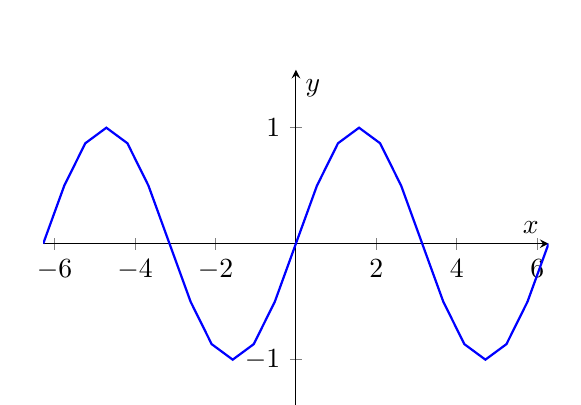
\begin{tikzpicture}
    \begin{axis}[
        axis lines=middle,
        xlabel=$x$,
        ylabel=$y$,
        xmin=-2*pi, xmax=2*pi,
        ymin=-1.5, ymax=1.5,
        width=8cm, height=6cm
    ]
    \addplot[domain=-2*pi:2*pi, blue, thick] {sin(deg(x))};
    \end{axis}
\end{tikzpicture}

\section{題庫}
\begin{enumerate}[label=\arabic*.]
    % 計算題 (10)
    \item 求$\sin 135^\circ$。
    \item 求$\cos 300^\circ$。
    \item $y = 3 \sin(2x)$,求週期。
    \item $\sin 30^\circ \cos 60^\circ$。
    \item $\sin 45^\circ + \sin 15^\circ$。
    \item 求$\cos 120^\circ$。
    \item $y = 2 \cos(4x)$,求振幅。
    \item $\cos 60^\circ \cos 30^\circ$。
    \item $\sin 75^\circ - \sin 15^\circ$。
    \item $\sin \theta \sin 2\theta$,化簡。
    % 應用題 (20)
    \item 求$\sin 105^\circ$。
    \item $y = 4 \sin(3x - \pi)$,求週期。
    \item 化簡$\cos 45^\circ \sin 15^\circ$。
    \item 一波$y = 5 \sin(2t)$,求最大值。
    \item 求$\sin x = \frac{\sqrt{3}}{2}$,$0 \leq x < 2\pi$。
    \item 化簡$\sin 75^\circ + \sin 45^\circ$。
    \item $y = 2 \cos(3x + \frac{\pi}{2})$,求週期。
    \item 化簡$\sin 60^\circ \sin 30^\circ$。
    \item 一物振動$y = 3 \sin(4t)$,求頻率。
    \item 求$\cos 15^\circ - \cos 75^\circ$。
    \item $\cos x = -\frac{1}{2}$,$0 \leq x < 2\pi$。
    \item $y = 5 \sin(2x - \frac{\pi}{4})$,求相位移。
    \item 化簡$\cos 105^\circ + \cos 15^\circ$。
    \item 波動$y = 4 \cos(5t)$,求週期。
    \item 求$\sin 285^\circ$。
    \item $\sin 2\theta \cos \theta$,化簡。
    \item $y = 3 \sin(2x + \pi)$,求振幅。
    \item 化簡$\sin 165^\circ - \sin 105^\circ$。
    \item 一鐘擺$y = 2 \cos(6t)$,求週期。
    \item 求$\sin 45^\circ \cos 15^\circ + \cos 45^\circ \sin 15^\circ$。
    % 觀念題 (10)
    \item 積化和差的用途?
    \item 和差化積如何推導?
    \item 證明$\sin \alpha \cos \beta = \frac{1}{2} [\sin(\alpha + \beta) + \sin(\alpha - \beta)]$。
    \item $\sin^2 \theta + \cos^2 \theta = 1$的意義?
    \item 證明$\sin \alpha + \sin \beta = 2 \sin\left(\frac{\alpha + \beta}{2}\right) \cos\left(\frac{\alpha - \beta}{2}\right)$。
    \item 週期如何定義?
    \item 證明$\cos \alpha \cos \beta = \frac{1}{2} [\cos(\alpha + \beta) + \cos(\alpha - \beta)]$。
    \item 相位移的作用?
    \item 證明$\cos \alpha - \cos \beta = -2 \sin\left(\frac{\alpha + \beta}{2}\right) \sin\left(\frac{\alpha - \beta}{2}\right)$。
    \item 二倍角公式的應用?
    % 進階題 (10)
    \item 化簡$\sin 3\theta \cos \theta$。
    \item $y = 3 \sin(2x) + 4 \cos(2x)$,求振幅。
    \item 化簡$\cos 75^\circ - \cos 15^\circ$。
    \item 求$\cos x = 0$,$0 \leq x < 2\pi$。
    \item $y = 2 \sin(x - \frac{\pi}{3})$,求最小值。
    \item 化簡$\sin 135^\circ + \sin 45^\circ$。
    \item $\sin x + \cos x = 1$,$0 \leq x < 2\pi$。
    \item 化簡$\cos 30^\circ \sin 60^\circ$。
    \item $y = 5 \sin(3x + \frac{\pi}{6})$,求最大值。
    \item 求$\sin 105^\circ \cos 15^\circ$。
    % 挑戰題 (10)
    \item $y = \sin x + \cos x$,求振幅。
    \item 證明$\sin 3\theta = 3 \sin \theta - 4 \sin^3 \theta$。
    \item 化簡$\sin 120^\circ + \sin 60^\circ$。
    \item $y = 4 \sin(2x) - 3 \cos(2x)$,求振幅。
    \item 化簡$\cos 255^\circ - \cos 105^\circ$。
    \item $\sin 2x = \cos x$,$0 \leq x < 2\pi$。
    \item 證明$\cos 2\theta \sin \theta = \frac{1}{2} [\sin 3\theta - \sin \theta]$。
    \item $y = 3 \sin(4x + \frac{\pi}{2})$,求最小值。
    \item 化簡$\sin 75^\circ \cos 45^\circ + \cos 75^\circ \sin 45^\circ$。
    \item 求$\cos 135^\circ + \cos 45^\circ$。
\end{enumerate}


\chapter{平面向量}
\section{觀念與公式}

\subsection{基本概念}
向量表示大小與方向。\\
\textbf{定義}:
\begin{itemize}
    \item 幾何向量:箭頭表示。
    \item 坐標向量:$\vec{v} = (x, y)$。
    \item 模:$|\vec{v}| = \sqrt{x^2 + y^2}$。
\end{itemize}
\textbf{應用}:位置表示。\\
\textbf{大學技巧}:線性空間定義。

\subsection{向量運算}
基本運算規則。\\
\textbf{公式}:
\begin{itemize}
    \item 加法:$\vec{a} + \vec{b} = (a_1 + b_1, a_2 + b_2)$。
    \item 減法:$\vec{a} - \vec{b} = (a_1 - b_1, a_2 - b_2)$。
    \item 數乘:$k\vec{a} = (ka_1, ka_2)$。
    \item 內積:$\vec{a} \cdot \vec{b} = a_1 b_1 + a_2 b_2 = |\vec{a}| |\vec{b}| \cos \theta$。
\end{itemize}
\textbf{應用}:方向與大小。\\
\textbf{大學技巧}:矩陣表示。

\subsection{向量性質}
幾何與代數性質。\\
\textbf{性質}:
\begin{itemize}
    \item 平行:$\vec{a} = k\vec{b}$。
    \item 垂直:$\vec{a} \cdot \vec{b} = 0$。
    \item 單位向量:$\hat{v} = \frac{\vec{v}}{|\vec{v}|}$。
\end{itemize}
\textbf{應用}:夾角計算。\\
\textbf{大學技巧}:投影。

\subsection{幾何應用}
向量在平面幾何中應用。\\
\textbf{公式}:
\begin{itemize}
    \item 中點向量:$\vec{M} = \frac{\vec{A} + \vec{B}}{2}$。
    \item 三角形面積:$S = \frac{1}{2} |\vec{a} \cdot \vec{b} \sin \theta|$(或行列式)。
\end{itemize}
\textbf{應用}:物理與測量。\\
\textbf{大學技巧}:外積$|\vec{a} \times \vec{b}|$。

\section{例題解析}

\subsection{例題1:基本運算}
$\vec{a} = (3, 4)$,$\vec{b} = (1, -2)$,求$\vec{a} + \vec{b}$與$|\vec{a}|$。\\
\textbf{解}:$\vec{a} + \vec{b} = (4, 2)$,$|\vec{a}| = \sqrt{3^2 + 4^2} = 5$。

\subsection{例題2:內積與夾角}
$\vec{a} = (1, 2)$,$\vec{b} = (3, -1)$,求$\vec{a} \cdot \vec{b}$與夾角。\\
\textbf{解}:$\vec{a} \cdot \vec{b} = 1 \cdot 3 + 2 \cdot (-1) = 1$。\\
$|\vec{a}| = \sqrt{5}$,$|\vec{b}| = \sqrt{10}$,$\cos \theta = \frac{1}{\sqrt{50}}$,$\theta = \cos^{-1}\left(\frac{1}{5\sqrt{2}}\right)$。

\subsection{例題3:平行與垂直}
判斷$\vec{a} = (2, -4)$與$\vec{b} = (-1, 2)$是否平行。\\
\textbf{解}:$\vec{a} = -2\vec{b}$,平行。

\subsection{例題4:幾何應用}
點$A(1, 1)$,$B(3, 5)$,求中點向量與$AB$長度。\\
\textbf{解}:$\vec{AB} = (2, 4)$,中點$\vec{M} = (2, 3)$,$|\vec{AB}| = \sqrt{20} = 2\sqrt{5}$。

\subsection{例題5:應用題}
力$\vec{F} = (3, 4)$沿$\vec{d} = (1, 1)$分解,求分量。\\
\textbf{解}:投影$|\vec{F}| \cos \theta = \frac{\vec{F} \cdot \vec{d}}{|\vec{d}|} = \frac{7}{\sqrt{2}}$,分量$\frac{7}{\sqrt{2}} \cdot \frac{\vec{d}}{|\vec{d}|} = \left(\frac{7}{2}, \frac{7}{2}\right)$。

\section{圖形展示}
向量加法:
\begin{tikzpicture}
    \draw[->] (0,0) -- (2,1) node[right] {$\vec{a}$};
    \draw[->] (2,1) -- (3,3) node[right] {$\vec{b}$};
    \draw[->, blue] (0,0) -- (3,3) node[above] {$\vec{a} + \vec{b}$};
\end{tikzpicture}

\section{題庫}
\begin{enumerate}[label=\arabic*.]
    % 計算題 (10)
    \item $\vec{a} = (2, 3)$,求$|\vec{a}|$。
    \item $\vec{a} = (1, -1)$,$\vec{b} = (2, 3)$,求$\vec{a} + \vec{b}$。
    \item $\vec{a} = (4, 0)$,求$2\vec{a}$。
    \item $\vec{a} = (3, 4)$,$\vec{b} = (-1, 2)$,求$\vec{a} \cdot \vec{b}$。
    \item $\vec{a} = (1, 1)$,求單位向量。
    \item $\vec{a} = (5, -2)$,求$|\vec{a}|$。
    \item $\vec{a} = (2, -1)$,$\vec{b} = (1, 2)$,求$\vec{a} - \vec{b}$。
    \item $\vec{a} = (0, 3)$,$\vec{b} = (4, 0)$,求夾角。
    \item $\vec{a} = (6, 8)$,求$|\vec{a}|$。
    \item $\vec{a} = (1, 2)$,$\vec{b} = (-2, 1)$,求$\vec{a} \cdot \vec{b}$。
    % 應用題 (20)
    \item $\vec{a} = (3, 1)$,$\vec{b} = (2, -2)$,求$\vec{a} + \vec{b}$與夾角。
    \item 點$A(2, 3)$,$B(5, 7)$,求$\vec{AB}$與長度。
    \item $\vec{a} = (1, 3)$,$\vec{b} = (-3, 9)$,判斷是否平行。
    \item $\vec{a} = (2, 1)$,$\vec{b} = (-1, 2)$,求是否垂直。
    \item 力$\vec{F} = (4, 3)$沿$\vec{d} = (1, 0)$,求分量。
    \item $\triangle ABC$,$A(0, 0)$,$B(2, 0)$,$C(1, 3)$,求面積。
    \item $\vec{a} = (5, 2)$,$\vec{b} = (1, -1)$,求$\vec{a} \cdot \vec{b}$與$\theta$。
    \item 點$P(1, 2)$,$Q(4, 6)$,求中點向量。
    \item $\vec{a} = (3, -2)$,分解成$\vec{b} = (1, 1)$方向的分量。
    \item $\vec{a} = (4, 0)$,$\vec{b} = (0, 3)$,求面積。
    \item $\vec{a} = (2, 5)$,$\vec{b} = (-1, 2)$,求$|\vec{a} + \vec{b}|$。
    \item 點$A(0, 1)$,$B(3, 4)$,求$|\vec{AB}|$。
    \item $\vec{a} = (1, -1)$,$\vec{b} = (2, 2)$,求夾角。
    \item $\vec{F} = (6, 8)$沿$\vec{d} = (3, 4)$,求分量大小。
    \item $\triangle ABC$,$A(1, 1)$,$B(3, 2)$,$C(2, 4)$,求面積。
    \item $\vec{a} = (2, -3)$,$\vec{b} = (4, 1)$,求$\vec{a} - \vec{b}$。
    \item 點$P(0, 0)$,$Q(2, 3)$,$R(4, 1)$,求$\vec{PQ} + \vec{PR}$。
    \item $\vec{a} = (5, 0)$,$\vec{b} = (0, 5)$,求是否垂直。
    \item $\vec{a} = (3, 4)$,求單位向量。
    \item $\vec{a} = (1, 2)$,$\vec{b} = (3, -1)$,求$2\vec{a} - \vec{b}$。
    % 觀念題 (10)
    \item 向量模的意義?
    \item 內積如何判斷垂直?
    \item 平行向量的條件?
    \item 向量加法的幾何意義?
    \item 單位向量的定義?
    \item 內積與夾角的關係?
    \item 如何用向量求面積?
    \item 數乘向量的效果?
    \item 向量分解的原理?
    \item 中點向量的公式?
    % 進階題 (10)
    \item $\vec{a} = (2, 3)$,$\vec{b} = (1, -2)$,求投影分量於$\vec{b}$。
    \item $\triangle ABC$,$A(0, 0)$,$B(4, 0)$,$C(2, 3)$,求面積。
    \item $\vec{a} = (3, 1)$,$\vec{b} = (-2, 4)$,求$\theta$。
    \item $\vec{a} = (5, 2)$,分解成$\vec{b} = (1, 1)$與垂直分量。
    \item $\vec{a} = (1, 1)$,$\vec{b} = (2, -2)$,求$|\vec{a} + \vec{b}|$。
    \item 點$A(1, 2)$,$B(3, 5)$,$C(4, 1)$,求$\vec{AB} \cdot \vec{AC}$。
    \item $\vec{a} = (4, -3)$,$\vec{b} = (2, 1)$,求面積。
    \item $\vec{F} = (6, 8)$沿$\vec{d} = (1, 0)$,求分量與垂直分量。
    \item $\vec{a} = (2, 5)$,$\vec{b} = (-1, 3)$,求$3\vec{a} - 2\vec{b}$。
    \item $\triangle ABC$,$A(0, 0)$,$B(2, 2)$,$C(4, 0)$,求中點$M$向量。
    % 挑戰題 (10)
    \item $\vec{a} = (3, 4)$,$\vec{b} = (1, -1)$,求$\vec{a}$在$\vec{b}$上的投影向量。
    \item $\triangle ABC$,$A(0, 0)$,$B(3, 0)$,$C(0, 4)$,求面積與$\vec{AC}$單位向量。
    \item $\vec{a} = (2, 1)$,$\vec{b} = (-1, 2)$,求$\vec{a} + \vec{b}$與面積。
    \item $\vec{F} = (5, 5)$分解成$\vec{d} = (1, 0)$與垂直分量。
    \item 點$A(1, 1)$,$B(4, 3)$,$C(2, 5)$,求面積。
    \item $\vec{a} = (3, -2)$,$\vec{b} = (4, 1)$,求$\vec{a} \cdot \vec{b}$與$\theta$。
    \item $\vec{a} = (1, 2)$,$\vec{b} = (2, 1)$,求$|\vec{a} - \vec{b}|$與夾角。
    \item $\triangle ABC$,$A(0, 0)$,$B(5, 0)$,$C(2, 4)$,求面積。
    \item $\vec{a} = (4, 3)$,$\vec{b} = (-2, 5)$,求投影與垂直分量於$\vec{b}$。
    \item 點$P(0, 0)$,$Q(2, 3)$,$R(4, 1)$,求$\vec{PQ} \cdot \vec{PR}$。
\end{enumerate}

\chapter{空間向量}
\input{src/chapter12.tex}

\chapter{空間中平面與直線方程式}
\input{src/chapter13.tex}

\chapter{矩陣}
\input{src/chapter14.tex}

\chapter{題庫解答}
\section{CH1題庫解答}
\begin{enumerate}[label=\arabic*.]
    % 計算題
    \item $(2 + 3i) + (4 - 5i) = 6 - 2i$。
    \item $|5 - 2i| = \sqrt{5^2 + (-2)^2} = \sqrt{29}$。
    \item $|x - 2| = 3 \implies x = 5 \text{或} -1$。
    \item $\frac{1 + i}{1 - i} \cdot \frac{1 + i}{1 + i} = \frac{2i}{2} = i$。
    \item $(1 + i)^2 = 2i$,$(1 + i)^3 = 2i(1 + i) = -2 + 2i$。
    \item $|2x + 1| = 5 \implies x = 2 \text{或} -3$。
    \item $|-3 + 4i|^2 = 9 + 16 = 25$。
    \item $\sqrt{18} = 3\sqrt{2}$,$\sqrt{50} = 5\sqrt{2}$,和為$8\sqrt{2}$。
    \item $|x + 3| = |x - 1|$,分段得$x = -1$。
    \item $\sqrt{5 + 12i}$模為$\sqrt{5^2 + 12^2} = 13$。
    % 應用題
    \item $3 < x < 7$。
    \item $ab \leq 36$,$a = b = 6$時為36。
    \item $|10 - x|$。
    \item $\frac{8}{ab}$,$ab \leq 16$,最小值$0.5$($a = b = 4$)。
    \item $90 \leq x \leq 110$。
    \item $|x| + |y| \leq 2$,$x = y = 1$時為2。
    \item $1 < x < 5$。
    \item $abc \leq 125$,$a = b = c = 5$時為125。
    \item $x < 0.5$。
    \item $a + b \leq 2\sqrt{2}$,$a = b = \sqrt{2}$時達成。
    % 觀念題
    \item $(x + y)^2 \leq (|x| + |y|)^2$,得證。
    \item $x = 0$。
    \item $a = b$。
    \item 是,因$|z| = |\overline{z}|$。
    \item $x$到$a$的距離小於$b$。
    \item $|x| \leq |x - y| + |y|$,同理得證。
    \item $\frac{a + b}{2} \geq \sqrt{ab}$。
    \item 是,因$|-z| = |z|$。
    \item 否,如$x = 1, y = -1$。
    \item $(a - b)^2 \geq 0$,整理得證。
    % 進階題
    \item $x \in [-1, 1]$。
    \item 圓心$(1, 0)$,半徑2。
    \item $(a - b)^2 + (b - c)^2 + (c - a)^2 \geq 0$,得證。
    \item $x \in [2, 3]$。
    \item $\sqrt{2}$,$x = y = \frac{\sqrt{2}}{2}$。
    \item 實部為0。
    \item $x < -0.5$。
    \item 最小值50,$a = b = 5$。
    \item $2\sqrt{3} - 3\sqrt{3} + 5\sqrt{3} = 4\sqrt{3}$。
    \item $z$在實軸上。
    % 挑戰題
    \item $x \in [1, 4]$。
    \item 最小值0,$a = b = 3$。
    \item $(\sqrt{\frac{a}{b}} - \sqrt{\frac{b}{a}})^2 \geq 0$,得證。
    \item $z$在$x = y$直線上。
    \item 最小值3,$x = y = z = 1$。
    \item $x \in [-4, -2] \cup [0, 4]$。
    \item $z = 2 \pm i\sqrt{3}$。
    \item $(a - 2b)^2 + (2b)^2 \geq 0$,$a = 2b$時成立。
    \item $x = 0$。
    \item 最小值9,$a = b = c = 1$。
    \item 2個解。
    \item 最小值0,$x = y = 0$。
    \item 用AM-GM與HM-GM證。
    \item $x \in [0, 4]$。
    \item 橢圓。
    \item $\sqrt{2}$。
    \item 最小值27,$a = b = c = 3$。
    \item $x = -\frac{1}{3}$。
    \item 最大值4。
    \item $2 + i$(模為$\sqrt{10}$)。
\end{enumerate}
\section{CH2題庫解答}
\begin{enumerate}[label=\arabic*.]
    % 計算題
    \item $y + 2 = 3(x - 1) \implies 3x - y - 5 = 0$。
    \item $(x + 1)^2 + (y - 2)^2 = 9$,中心$(-1, 2)$,半徑$3$。
    \item $m = \frac{2}{3}$,$y$截距$2$。
    \item $y = \frac{4}{3}x$。
    \item 中心$(1, -2)$,半徑$3$。
    \item $d = \frac{|2 + 1 - 3|}{\sqrt{2}} = 0$。
    \item $x^2 + (2x)^2 = 1 \implies 5x^2 = 1$,$\Delta > 0$,相交。
    \item $m = 2$,$2x - y - 1 = 0$。
    \item $x = 2$,$y = \pm 2$,交點$(2, 2)$與$(2, -2)$。
    \item $d = \frac{|0 - 20 + 10|}{\sqrt{25}} = 2$。
    % 應用題
    \item 垂足$(1, 2)$,距離$\sqrt{2}$。
    \item $x^2 + y^2 = 25$。
    \item $d = \sqrt{13}$,$m = \pm \frac{2}{3}$。
    \item 垂線$y = x$,交點$\left(\frac{1}{2}, \frac{1}{2}\right)$。
    \item $(x - 1)^2 + y^2 = 2$。
    \item $x = 1$,交點$(1, 1)$。
    \item $|k| < \sqrt{2}$。
    \item $y = \pm x + 3$。
    \item 如$(1, 2)$,滿足條件。
    \item $x = 1 + 2\cos\theta$,$y = 1 + 2\sin\theta$,$m = 1$時,點$\left(1 + \sqrt{2}, 1 - \sqrt{2}\right)$。
    % 觀念題
    \item 內積為0,得證。
    \item 無實數解,空集。
    \item $\Delta < 0$。
    \item 垂線長度。
    \item 2個。
    \item 切線與半徑內積為0。
    \item 平行。
    \item 相切。
    \item 方向向量參數化。
    \item 法向量垂直於直線。
    % 進階題
    \item $x = 1 \pm \sqrt{2}$,交點$\left(1 + \sqrt{2}, -\sqrt{2} - 1\right)$,$\left(1 - \sqrt{2}, -\sqrt{2} + 1\right)$。
    \item $y = -x$。
    \item $x + y - 5 = 0$。
    \item $\left(-\frac{\sqrt{2}}{2}, \frac{\sqrt{2}}{2}\right)$。
    \item $|k| < 5$。
    \item $x = 1$。
    \item $2\sqrt{5}$。
    \item 不存在(半徑矛盾)。
    \item $\left(\frac{1}{2}, \frac{1}{2}\right)$,$\left(\frac{1}{2}, \frac{1}{2}\right)$。
    \item 切點到圓心等於半徑。
    % 挑戰題
    \item $y = x - 2$,$y = -x + 2$。
    \item $|m| < \sqrt{3}$。
    \item 垂足$\left(\frac{12}{13}, \frac{18}{13}\right)$,距離$\frac{9}{\sqrt{13}}$。
    \item $2$。
    \item $a^2 + b^2 = 1$。
    \item $|m - 1| < 1$。
    \item $(1 + \sqrt{3}, 1 + \sqrt{3})$,$(1 - \sqrt{3}, 1 - \sqrt{3})$。
    \item $x^2 + y^2 = 2$。
    \item $3x - y - 1 = 0$,交點$\left(\frac{5}{2}, -\frac{1}{2}\right)$。
    \item $|m| > 1$。
    \item $\left(\sqrt{5} \cdot \frac{-1}{\sqrt{2}}, \sqrt{5} \cdot \frac{1}{\sqrt{2}}\right)$。
    \item $k = \pm 2$。
    \item $y = x$。
    \item $k = \pm 2$。
    \item $2\sqrt{2}$。
    \item $|m| < 1$。
    \item 垂足$\left(\frac{8}{5}, \frac{4}{5}\right)$,距離$\frac{4}{\sqrt{5}}$。
    \item $(x - 1)^2 + (y - 1)^2 = 2$。
    \item $(1 + \sqrt{2}, -1 + 2\sqrt{2})$,$(1 - \sqrt{2}, -1 - 2\sqrt{2})$。
    \item $|m| < \sqrt{3}$。
\end{enumerate}

\section{CH3題庫解答}
\begin{enumerate}[label=\arabic*.]
    % 計算題
    \item $x^3 - x^2 - x + 1$。
    \item $(x - 2)(x^2 + 2x + 4)$。
    \item $P(1) = -1$。
    \item $(x - 2)(x + 2)(x^2 + 4)$。
    \item $P(2) = 5$。
    \item 商$x^2 - 2x + 1$,餘數$0$。
    \item $(x - 2)^2$。
    \item $P(0) = 1$,$P'(0) = -1$,$1 - x$。
    \item $P(-1) = -4$。
    \item $(x + 3)(x^2 - 3x + 9)$。
    % 應用題
    \item $x = 1$(三重根)。
    \item $\sum r_i = 5$,$k = 8$。
    \item $P(0) = 1$。
    \item $P(x) = x^2 - x$。
    \item $x = 0, \pm \sqrt{3}$。
    \item $6$。
    \item $P(0) = -1$。
    \item $(-\infty, -5)$減,$(-5, 1)$增,$(1, \infty)$減。
    \item $x \to \infty$,$P(x) \to \infty$。
    \item $x = 0, \sqrt{3}, -\sqrt{3}$。
    % 觀念題
    \item 用多項式除法證。
    \item $P'(a) = 0$。
    \item 求未知係數。
    \item $0, 1, 2, 3$。
    \item $P^{(n+1)}(x) = 0$。
    \item $P(a) = 0$。
    \item $a_n < 0$且$n$為奇數。
    \item $P'(x) > 0$,單調增。
    \item $n$階差商為常數。
    \item $rx + s$。
    % 進階題
    \item $x = 1, 2$。
    \item $x = 0, \pm 1$。
    \item $x = 1$(二重根)。
    \item $x^2 - x$。
    \item $P(1) = 0$,$P'(1) = 3$,$3(x - 1)$。
    \item $x = \frac{2 \pm \sqrt{2}}{3}$。
    \item $x = 1$,1個。
    \item $x \to \infty$,$P(x) \to \infty$。
    \item $P(x) = x^2 + 1$。
    \item $x = 1$(二重根),$2$。
    % 挑戰題
    \item $x = \pm \sqrt{3}$,極值$3, -\frac{9}{4}$。
    \item $(x - 1)^3$。
    \item 3個。
    \item $P(3) = 2$。
    \item $x = \pm \sqrt{3}$,極值$-3, 0$。
    \item $x = -1, 2, 3$。
    \item 商$x^3 - 2x^2 + 1$,餘數$0$。
    \item $P(-1) = -2$。
    \item $x = 1, 2, 3$,和$6$,乘積$6$。
    \item $P(x) = x^2 + 1$。
    \item $x = 1$,極值$0$。
    \item $P(1) = -1$。
    \item $(-\sqrt{2}, \sqrt{2})$減。
    \item $P(2) = 3$。
    \item $x = \frac{2}{3}$。
    \item $0 + 2(x - 1) + 3(x - 1)^2$。
    \item $x \to \infty$,$P(x) \to \infty$。
    \item $x = -1, 2, 3$。
    \item $x^2 - 2x - 1$。
    \item $P(1) = -1$。
\end{enumerate}

\section{CH4解答}
\begin{enumerate}[label=\arabic*.]
    % 計算題
    \item $a_{10} = 5 + 9 \cdot 3 = 32$。
    \item $S_5 = 2 \frac{1 - 2^5}{1 - 2} = 62$。
    \item $S_{10} = 195$。
    \item $d = 2$。
    \item $a_6 = 3 \cdot \left(\frac{1}{2}\right)^5 = \frac{3}{32}$。
    \item $S_{20} = 10 \cdot (2 - 19) = -170$。
    \item $a_8 = 1 + 7 \cdot 3 = 22$。
    \item $S_4 = 1 \cdot \frac{1 - (-2)^4}{1 - (-2)} = -5$。
    \item $a_{15} = 10 + 14 \cdot 2 = 38$。
    \item $S_\infty = \frac{4}{1 - 0.5} = 8$。
    % 應用題
    \item $S_{10} = 5 \cdot (1000 + 2800) = 19000$元。
    \item $S_\infty = 10 + 2 \cdot 10 \cdot \frac{0.8}{1 - 0.8} = 90$公尺。
    \item $S_6 = 1 \cdot \frac{1 - 2^6}{1 - 2} = 63$。
    \item $n = 9$。
    \item $S_5 = 5000 \cdot \frac{1 - 0.9^5}{0.1} \approx 19531$元。
    \item $a_n = 6n - 3$。
    \item $d = 2$。
    \item $r = 2$。
    \item $a_5 = 15$。
    \item $S_\infty = \frac{5}{1 - \frac{1}{3}} = 7.5$。
    % 觀念題
    \item 用歸納法證。
    \item 不存在。
    \item 基礎步與歸納步。
    \item $a_n = 2n - 1$。
    \item 用幾何級數求和。
    \item 兩種。
    \item $S_n = 2^n - 1$。
    \item $a_n = a_{n-1} + a_{n-2}$。
    \item $a_n = 2n$。
    \item $|r| < 1$。
    % 進階題
    \item $n = 7$。
    \item $a_5 = 162, S_5 = 242$。
    \item $a_7 = 13$。
    \item $a_n = 2^{n-1}$。
    \item $n = 8$。
    \item $n = 7$。
    \item $S_{10} = 255$。
    \item $S_{100} = 0$。
    \item $S_5 = 195$。
    \item $a_6 = 243$。
    % 挑戰題
    \item $S_{10} = 110$。
    \item $n = 10$。
    \item $n = 8$。
    \item $n = 6$。
    \item $a_5 = 31$。
    \item $a_n = n^2$。
    \item $S_6 = -21$。
    \item $n = 10$。
    \item $S_{10} = 1023$。
    \item $S_8 = 92$。
    \item $n = 4$。
    \item $a_{20} = 77, S_{20} = 790$。
    \item $S_5 = 55$。
    \item $S_\infty = 15$。
    \item $S_{15} = 0$。
    \item $a_8 = 21$。
    \item $S_{10} \approx 65.6$。
    \item $n = 22$。
    \item $S_{10} = 125$。
    \item $n = 7$。
\end{enumerate}

\section{CH5題庫解答}
\begin{enumerate}[label=\arabic*.]
    % 計算題
    \item $3^{-1} = \frac{1}{3}$。
    \item $2$。
    \item $\log_5 3125 = 5$。
    \item $2$。
    \item $4$。
    \item $8$。
    \item $-3$。
    \item $10$。
    \item $3$。
    \item $125$。
    % 應用題
    \item $x = 4$。
    \item $1000 \cdot (1.05)^5 \approx 1276.28$元。
    \item $x = 10$。
    \item $0.933$,約6.7\%。
    \item $x = 4$。
    \item $a = 2$。
    \item $t \approx 35$年。
    \item $x = 2$。
    \item $pH = 7$。
    \item $x = 1.5$。
    % 觀念題
    \item 由定義證。
    \item $a > 1$增,$0 < a < 1$減。
    \item 用指數形式證。
    \item $x = y$。
    \item $x > 0$。
    \item 用指數形式證。
    \item $b = a^c$。
    \item $\log_a b = \frac{\ln b}{\ln a}$。
    \item 互為反函數,鏡像對稱。
    \item $(-\infty, \infty)$。
    % 進階題
    \item $x \approx 1.585$。
    \item $x = 2$。
    \item $9 + 9 \ln 3 (x - 2)$。
    \item $x = 1.5$。
    \item $a = 10$。
    \item $t \approx 6.93$小時。
    \item $x \approx 2.29$。
    \item $x = \pm 9$。
    \item $x = 3$。
    \item $\frac{1}{x} = 1$。
    % 挑戰題
    \item $x \approx 2.27$。
    \item $x = 3$。
    \item $x - \frac{x^2}{2} + \frac{x^3}{3}$。
    \item $x \approx 1.585$。
    \item $a = 9$。
    \item $t \approx 0.63$小時。
    \item $x = 1, 2$。
    \item $x = 2$。
    \item $x = 4$。
    \item $\ln 2$。
    \item $x \approx 1.76$。
    \item $x = 11$。
    \item $1 + x + \frac{x^2}{2}$。
    \item $x = 1$。
    \item $a > 0$(恆等)。
    \item $2593.74$人。
    \item $x \approx 0.96$。
    \item $x = \pm 6$。
    \item $x = 5$。
    \item $\frac{1}{9 \ln 3}$。
\end{enumerate}

\section{排組題庫解答}
\begin{enumerate}[label=\arabic*.]
    % 計算題
    \item $60$。
    \item $15$。
    \item $24$。
    \item $\frac{3!}{2!} = 3$。
    \item $24$。
    \item $42$。
    \item $56$。
    \item $\frac{3!}{2!} = 3$。
    \item $(4-1)! = 6$。
    \item $5$。
    % 應用題
    \item $5! \cdot 2 / 2 = 48$。
    \item $\binom{5}{2} = 10$。
    \item $(4-1)! - 2 \cdot 2 = 2$。
    \item $\binom{8}{4} \cdot \binom{4}{2} / 2 = 210$。
    \item $2^5 - 1^5 = 31$。
    \item $3^6 = 729$。
    \item $\binom{8}{4} - \binom{5}{4} = 65$。
    \item $240$。
    \item $\frac{5!}{2} = 60$。
    \item $\binom{7}{3} - \binom{4}{3} = 31$。
    \item $(3-1)! = 2$。
    \item $3! + 3! + 2! = 14$。
    \item $\binom{4}{2} + \binom{6}{3} = 26$。
    \item $\binom{5}{1} = 5$。
    \item $4^3 = 64$。
    \item $6! \cdot 2 / 2 \cdot \frac{6!}{2} / 2 = 8640$。
    \item $14$。
    \item $P(6, 3) - P(5, 2) = 110$。
    \item $\binom{8}{4} \cdot \binom{4}{2} / 2 = 210$。
    \item $P(5, 3) - 2 \cdot P(4, 2) = 36$。
    % 觀念題
    \item $k!(n-k)! = (n-k)!k!$。
    \item 固定一點,減1自由度。
    \item 用組合定義證。
    \item $\frac{n!}{n_1! n_2! \cdots n_k!}$。
    \item 找$k$次項係數。
    \item 不越$y=x$的路徑。
    \item $n^k$。
    \item 逐步選取證。
    \item 排列有序,組合無序。
    \item $2^n$。
    % 進階題
    \item $1 \cdot P(5, 2) = 20$。
    \item $540$。
    \item $\frac{5!}{2! 1! 1! 1!} = 60$。
    \item $42$。
    \item $\binom{6}{2} = 15$。
    \item $-567$。
    \item $6! - 3 \cdot 5! + 3 \cdot 4! = 312$。
    \item $5^4 - 4^4 = 369$。
    \item $5! \cdot 4 = 480$。
    \item $\binom{4}{3} + \binom{5}{2} = 14$。
    % 挑戰題
    \item $5! - 4! = 96$。
    \item $240$。
    \item $3^5 - 2^5 = 211$。
    \item $\frac{6!}{3! 2! 1!} = 60$。
    \item $\binom{7}{2} \binom{3}{2} + \binom{7}{3} \binom{3}{1} = 168$。
    \item $4! \cdot 3 = 72$。
    \item $1792$。
    \item $\binom{6}{1} + \binom{5}{1} = 11$。
    \item $\frac{5!}{2} \cdot \frac{4!}{2} = 720$。
    \item $\binom{10}{2} + \binom{10}{1} \binom{8}{1} + \binom{10}{5} = 341$。
\end{enumerate}

\section{數據分析題庫解答}
\begin{enumerate}[label=\arabic*.]
    % 計算題
    \item $6$。
    \item $6$。
    \item $1$。
    \item $10$。
    \item $2$。
    \item $5$。
    \item $24$。
    \item $20$。
    \item $2.8$。
    \item $1.22$。
    % 應用題
    \item $150, 152.5, 160, 167.5, 170$。
    \item $5.48$。
    \item 無離群值。
    \item $1$。
    \item $5.5$。
    \item $25, 10$。
    \item 對稱。
    \item $1$。
    \item $150, 167.5$。
    \item $70$,無離群值。
    \item $1000$。
    \item $-1$。
    \item $40, 50, 60, 75, 90$。
    \item $7.07$。
    \item $32.5, 15$。
    \item $y = 0.2x + 6$。
    \item $50$。
    \item $40, 70$。
    \item $7$,略。
    \item $1$。
    % 觀念題
    \item 平均數受極值影響,中位數不受。
    \item 標準差越大,分散越大。
    \item 最小、$Q_1$、中位數、$Q_3$、最大。
    \item $-1 \leq r \leq 1$,正負相關。
    \item 平均數 > 中位數。
    \item 全距整體,IQR中間50\%。
    \item 差平方平均。
    \item 點分佈趨勢。
    \item $Q_1-1.5IQR$或$Q_3+1.5IQR$外。
    \item 鐘形,68-95-99.7。
    % 進階題
    \item $1$。
    \item $2$。
    \item $2.5$。
    \item $y = 0.5x - 30$。
    \item $40, (-10, 70)$。
    \item $68\%$。
    \item $1$。
    \item $4.74$。
    \item $1$。
    \item $y = 5x + 145$。
    % 挑戰題
    \item $s=3.16, \sigma=2.83$。
    \item $200$。
    \item $97.5\%$。
    \item $1$。
    \item $r=1, y=x-110$。
    \item $8.25, 40$。
    \item $50, 1$。
    \item $y = \frac{2}{3}x + 50$。
    \item $略, 近似常態$。
    \item $0.97$。
\end{enumerate}

\section{機率題庫解答}
\begin{enumerate}[label=\arabic*.]
    % 計算題
    \item $\frac{1}{6}$。
    \item $\frac{3}{5}$。
    \item $\frac{1}{6}$。
    \item $\frac{1}{4}$。
    \item $\frac{3}{4}$。
    \item $\frac{4}{7}$。
    \item $\frac{1}{2}$。
    \item $\frac{1}{4}$。
    \item $3.5$。
    \item $\frac{2}{5}$。
    % 應用題
    \item $\frac{9}{49}$。
    \item $\frac{2}{5}$。
    \item $\frac{1}{2}$。
    \item $\frac{15}{56}$。
    \item $\frac{4}{663}$。
    \item $\frac{4}{5}$。
    \item $\frac{4}{15}$。
    \item $\frac{3}{8}$。
    \item $\frac{1}{3}$。
    \item $\frac{26}{36}$。
    \item $\frac{15}{36}$。
    \item $\frac{13}{20}$。
    \item $\frac{4}{5}$。
    \item $\frac{15}{28}$。
    \item $0.5$。
    \item $\frac{15}{28}$。
    \item $\frac{1}{2}$。
    \item $\frac{127}{219}$。
    \item $1$。
    \item $\frac{1}{12}$。
    % 觀念題
    \item 所有可能結果集合。
    \item $P(A \cup B) = P(A) + P(B)$。
    \item $P(A \cap B) = P(A) \cdot P(B)$。
    \item $P(A|B) = \frac{P(A \cap B)}{P(B)}$。
    \item $P(\overline{A}) = 1 - P(A)$。
    \item 理論vs頻率。
    \item 計數樣本空間。
    \item 隨機變量平均值。
    \item $0 \leq P \leq 1$。
    \item 分步計算。
    % 進階題
    \item $\frac{1}{3}$。
    \item $\frac{1}{5}$。
    \item $\frac{1}{20}$。
    \item $\frac{50}{125}$。
    \item $\frac{26}{51}$。
    \item $1.5$。
    \item $\frac{4}{7}$。
    \item $\frac{1}{7}$。
    \item $\frac{11}{30}$。
    \item $1.2$。
    % 挑戰題
    \item $\frac{7}{10}$。
    \item $\frac{1}{5}$。
    \item $\frac{2}{7}$。
    \item $\frac{148}{243}$。
    \item $3.75$。
    \item $\frac{48}{1275}$。
    \item $\frac{27}{56}$。
    \item $\frac{25}{216}$。
    \item $\frac{5}{12}$。
    \item $7$。
\end{enumerate}

\section{三角比題庫解答}
\begin{enumerate}[label=\arabic*.]
    % 計算題
    \item $4\sqrt{2}$。
    \item $10$。
    \item $14$。
    \item $\sqrt{11}$。
    \item $10$。
    \item $6$。
    \item $11\sqrt{3}$。
    \item $5$。
    \item $10.5$。
    \item $\frac{7}{2\sqrt{3}}$。
    % 應用題
    \item $7$。
    \item $3\sqrt{2}$。
    \item $25\sqrt{6}$。
    \item $11$。
    \item $6\sqrt{3}$。
    \item $\cos^{-1}(\frac{7}{8})$。
    \item $7\sqrt{2}$。
    \item $20$。
    \item $6, \frac{2\sqrt{2}}{3}$。
    \item $6\sqrt{6}$。
    \item $5\sqrt{3}$。
    \item $14\sqrt{3}$。
    \item $6$。
    \item $10$。
    \item $5$。
    \item $9\sqrt{2}$。
    \item $15$。
    \item $8$。
    \item $\frac{6}{\sqrt{3}}$。
    \item $60$。
    % 觀念題
    \item $S = \frac{1}{2}bc \sin A$,推$\frac{a}{\sin A} = 2R$。
    \item 直角三角形延伸證。
    \item 底$\cdot$高證。
    \item $\sin 60^\circ = \frac{\sqrt{3}}{2}, \cos 60^\circ = \frac{1}{2}$。
    \item $\frac{a}{\sin A} = \frac{b}{\sin B}$證。
    \item $\cos A = \frac{b^2 + c^2 - a^2}{2bc}$。
    \item 三邊平分證。
    \item $2R = \frac{a}{\sin A}$。
    \item 餘弦定理推$S$。
    \item $\vec{AB} \cdot \vec{AC}$證。
    % 進階題
    \item $\cos^{-1}(\frac{13}{28})$。
    \item $8$。
    \item $\sqrt{13}, \frac{5}{2}$。
    \item $20\sqrt{15}, \frac{20\sqrt{15}}{21}$。
    \item $11\sqrt{3}$。
    \item $\sin^{-1}(\frac{5}{6})$。
    \item $7\sqrt{2}, \frac{7\sqrt{2}}{2}$。
    \item $15$。
    \item $3\sqrt{3}$。
    \item $\sqrt{29}, 14\sqrt{2}$。
    % 挑戰題
    \item $\cos^{-1}(\frac{3}{14}), \frac{7}{2\sqrt{3}}$。
    \item $5\sqrt{2}$。
    \item $\sin^{-1}(\frac{4}{5}), \frac{8}{3}$。
    \item $24, 4$。
    \item $22.5^\circ, \frac{5\sqrt{3}}{2}$。
    \item $\frac{9}{4\sqrt{5}}, 28\sqrt{5}$。
    \item $6, 10$。
    \item $6\sqrt{2}, 6$。
    \item $55\sqrt{11}, \frac{55\sqrt{11}}{33}$。
    \item 角平分線證。
\end{enumerate}

\section{三角函數題庫解答}
\begin{enumerate}[label=\arabic*.]
    % 計算題
    \item $\frac{\sqrt{2}}{2}$。
    \item $\frac{1}{2}$。
    \item $\pi$。
    \item $\frac{\sqrt{3}}{4}$。
    \item $\frac{\sqrt{6}}{2}$。
    \item $-\frac{1}{2}$。
    \item $2$。
    \item $\frac{\sqrt{3}}{4}$。
    \item $\frac{\sqrt{2}}{2}$。
    \item $\frac{1}{2} [\cos \theta - \cos 3\theta]$。
    % 應用題
    \item $\frac{\sqrt{6} + \sqrt{2}}{4}$。
    \item $\frac{2\pi}{3}$。
    \item $\frac{\sqrt{6} - \sqrt{2}}{8}$。
    \item $5$。
    \item $\frac{\pi}{3}, \frac{2\pi}{3}$。
    \item $\sqrt{2}$。
    \item $\frac{2\pi}{3}$。
    \item $\frac{\sqrt{3}}{4}$。
    \item $2$。
    \item $-\sqrt{2}$。
    \item $\frac{2\pi}{3}, \frac{4\pi}{3}$。
    \item $\frac{\pi}{8}$。
    \item $\frac{\sqrt{2}}{2}$。
    \item $\frac{2\pi}{5}$。
    \item $-\frac{\sqrt{6} + \sqrt{2}}{4}$。
    \item $\frac{1}{2} [\sin 3\theta + \sin \theta]$。
    \item $3$。
    \item $\frac{\sqrt{2}}{2}$。
    \item $\frac{\pi}{3}$。
    \item $\frac{\sqrt{3}}{2}$。
    % 觀念題
    \item 將乘積轉和差。
    \item 令$u = \frac{\alpha + \beta}{2}$等證。
    \item 用和差公式推。
    \item 單位圓性質。
    \item 用$\sin u \cos v$推。
    \item 重複間隔。
    \item 用$\cos(\alpha + \beta)$證。
    \item 平移圖形。
    \item 用$\sin(\alpha - \beta)$證。
    \item 化簡角度。
    % 進階題
    \item $\frac{1}{2} [\sin 4\theta + \sin 2\theta]$。
    \item $5$。
    \item $-\sqrt{2}$。
    \item $\frac{\pi}{2}, \frac{3\pi}{2}$。
    \item $-2$。
    \item $\sqrt{2}$。
    \item $0, \frac{\pi}{2}$。
    \item $\frac{\sqrt{3}}{4}$。
    \item $5$。
    \item $\frac{\sqrt{6}}{4}$。
    % 挑戰題
    \item $\sqrt{2}$。
    \item 用$\sin(2\theta + \theta)$。
    \item $\frac{3\sqrt{3}}{2}$。
    \item $5$。
    \item $-\frac{\sqrt{6}}{2}$。
    \item $\frac{\pi}{6}, \frac{5\pi}{6}$。
    \item 用積化和差證。
    \item $-3$。
    \item $1$。
    \item $0$。
\end{enumerate}

\section{平面向量題庫解答}
\begin{enumerate}[label=\arabic*.]
    % 計算題
    \item $\sqrt{13}$。
    \item $(3, 2)$。
    \item $(8, 0)$。
    \item $5$。
    \item $\left(\frac{\sqrt{2}}{2}, \frac{\sqrt{2}}{2}\right)$。
    \item $\sqrt{29}$。
    \item $(1, -3)$。
    \item $90^\circ$。
    \item $10$。
    \item $0$。
    % 應用題
    \item $(5, -1), \cos^{-1}\left(\frac{8}{\sqrt{10} \sqrt{5}}\right)$。
    \item $(3, 4), 5$。
    \item 是,$\vec{b} = -3\vec{a}$。
    \item 是,$\vec{a} \cdot \vec{b} = 0$。
    \item $(4, 0)$。
    \item $3$。
    \item $3, \cos^{-1}\left(\frac{3}{\sqrt{29} \sqrt{2}}\right)$。
    \item $(2.5, 4)$。
    \item $\left(\frac{1}{2}, \frac{1}{2}\right)$。
    \item $6$。
    \item $\sqrt{10}$。
    \item $3\sqrt{2}$。
    \item $\cos^{-1}\left(\frac{1}{\sqrt{5}}\right)$。
    \item $10$。
    \item $2.5$。
    \item $(-2, -4)$。
    \item $(6, 4)$。
    \item 是,$\vec{a} \cdot \vec{b} = 0$。
    \item $\left(\frac{3}{5}, \frac{4}{5}\right)$。
    \item $(-1, 5)$。
    % 觀念題
    \item 大小。
    \item $\vec{a} \cdot \vec{b} = 0$。
    \item $\vec{a} = k\vec{b}$。
    \item 平行四邊形。
    \item $\frac{\vec{v}}{|\vec{v}|}$。
    \item $\cos \theta = \frac{\vec{a} \cdot \vec{b}}{|\vec{a}| |\vec{b}|}$。
    \item 內積或行列式。
    \item 縮放大小。
    \item 投影分量。
    \item $\frac{\vec{A} + \vec{B}}{2}$。
    % 進階題
    \item $-\frac{4}{\sqrt{5}}$。
    \item $6$。
    \item $\cos^{-1}\left(-\frac{2}{\sqrt{10} \sqrt{20}}\right)$。
    \item $\left(\frac{7}{2}, \frac{7}{2}\right), \left(\frac{3}{2}, -\frac{3}{2}\right)$。
    \item $\sqrt{5}$。
    \item $5$。
    \item $11$。
    \item $(6, 0), (0, 8)$。
    \item $(8, 11)$。
    \item $(2, 1)$。
    % 挑戰題
    \item $\left(-\frac{1}{2}, \frac{1}{2}\right)$。
    \item $6, \left(0, \frac{4}{5}\right)$。
    \item $(1, 3), 7$。
    \item $(5, 0), (0, 5)$。
    \item $4$。
    \item $10, \cos^{-1}\left(\frac{10}{\sqrt{13} \sqrt{17}}\right)$。
    \item $1, 45^\circ$。
    \item $10$。
    \item $\left(\frac{7}{29}, \frac{35}{29}\right), \left(\frac{109}{29}, -\frac{14}{29}\right)$。
    \item $10$。
\end{enumerate}

\end{document}